%%%%%%%%%%%%%%%%%%%%%%%%%%%%%%%%%%%%%%%%%%%%%%%%%%%%%%%%%%%%%%%%%%%%%%%%%%%%%%%
%
% Tommy P. Keane
% Master of Science Thesis
% Department of Electrical and Microelectronic Engineering
% Rochester Institute of Technology
%
% April 2011
%
%
% Funded By: Lenel Systems Inc., A UTC Fire & Security Corporation
%
% Algorithm Intellectual Property Owned By: Lenel Systems Inc.
%
% http://www.tommypkeane.com
%
%%%%%%%%%%%%%%%%%%%%%%%%%%%%%%%%%%%%%%%%%%%%%%%%%%%%%%%%%%%%%%%%%%%%%%%%%%%%%%%


\documentclass[11pt]{report}
\usepackage{subfigure}
\usepackage[english]{babel}
\usepackage{times}
\usepackage{amssymb}
\usepackage{amsmath}
\usepackage{lscape}
\usepackage{verbatim}
\usepackage{enumerate}
\usepackage{afterpage}
\usepackage{subfigure}
\usepackage{graphicx}
\graphicspath{{./images/}}
\usepackage{RIT_EEME_MS_ThesisStyle}
\usepackage{setspace}


\bibliographystyle{unsrt}


%%%%%%%%%%%%%%%%%%%%%%%%%%%%%%%%%%%%%%%%%%%%%%%%%%%%%%%%%%%%%%%%%%%%%%%%%%%%%%%
% BEGIN DOCUMENT

\begin{document}



%%%%%%%%%%%%%%%%%%%%%%%%%%%%%%%%%%%%%%%%%%%%%%%%%%%%%%%%%%%%%%%%%%%%%%%%%%%%%%%
% USEFUL ABBREVIATIONS

\newcommand{\etc} {\emph{etc.\/}}
\newcommand{\etal}{\emph{et~al.\/}}
\newcommand{\eg}  {\emph{e.g.\/}}
\newcommand{\ie}  {\emph{i.e.\/}}




%%%%%%%%%%%%%%%%%%%%%%%%%%%%%%%%%%%%%%%%%%%%%%%%%%%%%%%%%%%%%%%%%%%%%%%%%%%%%%%
% TITLE
% The \title{} can contain line breaks as appropriate...

\title{\vspace{-0.20in}Weighted and Filtered Mutual Information:
   \\
   A metric for automated creation of panoramas from views of complex scenes}

% The \titleline{} must have no line breaks in it.
\titleline{Weighted and Filtered Mutual Information: A metric for automated creation of panoramas from views of complex scenes}

% There should be no reason to change the \thesistype{} or the \MSThesistrue...
\thesistype{Thesis}
\MSthesistrue





%%%%%%%%%%%%%%%%%%%%%%%%%%%%%%%%%%%%%%%%%%%%%%%%%%%%%%%%%%%%%%%%%%%%%%%%%%%%%%%
% AUTHOR
% The \author{} should be exactly the same as your diploma

\author{Thomas P. Keane}
\dept{Electrical and Microelectronic Engineering}




%%%%%%%%%%%%%%%%%%%%%%%%%%%%%%%%%%%%%%%%%%%%%%%%%%%%%%%%%%%%%%%%%%%%%%%%%%%%%%%
% COMMITTEE MEMBERS
% The following information is for the signature page.

\firstreader{REDACTED}{Professor}
	%{Electrical and Microelectronic Engineering}
\secondreader{REDACTED}{Professor}
	%{Imaging Science}
\thirdreader{REDACTED}{Professor}
	%{Computer Engineering}
\fourthreader{REDACTED}{Professor}
	%{Electrical and Microelectronic Engineering}





%%%%%%%%%%%%%%%%%%%%%%%%%%%%%%%%%%%%%%%%%%%%%%%%%%%%%%%%%%%%%%%%%%%%%%%%%%%%%%%
% DEFINE DATE

\grantdate{April}{2011}





%%%%%%%%%%%%%%%%%%%%%%%%%%%%%%%%%%%%%%%%%%%%%%%%%%%%%%%%%%%%%%%%%%%%%%%%%%%%%%%
% FRONT MATTER SETUP

\beforepreface





%%%%%%%%%%%%%%%%%%%%%%%%%%%%%%%%%%%%%%%%%%%%%%%%%%%%%%%%%%%%%%%%%%%%%%%%%%%%%%%
% DEDICATION

\prefacesection{Dedication}

%%%%%%%%%%%%%%%%%%%%%%%%%%%%%%%%%%%%%%%%%%%%%%%%%%%%%%%%%%%%%%%%%%%%%%%%%%%%%%%
%
% Tommy P. Keane
% Master of Science Thesis
% Department of Electrical and Microelectronic Engineering
%
% March 2011
%
%
%
%%%%%%%%%%%%%%%%%%%%%%%%%%%%%%%%%%%%%%%%%%%%%%%%%%%%%%%%%%%%%%%%%%%%%%%%%%%%%%%

%%%%%%%%%%%%%%%%%%%%%%%%%%%%%%%%%%%%%%%%%%%%%%%%%%%%%%%%%%%%%%%%%%%%%%%%%%%%%%%
%
% DEDICATION
%
%%%%%%%%%%%%%%%%%%%%%%%%%%%%%%%%%%%%%%%%%%%%%%%%%%%%%%%%%%%%%%%%%%%%%%%%%%%%%%%


%%%%%%%%%%%%%%%%%%%%%%%%%%%%%%%%%%%%%%%%%%%%%%%%%%%%%%%%%%%%%%%%%%%%%%%%%%%%%%%
% BEGIN DOCUMENT
\begin{center}

\vfill

\textit{[REDACTED; 2023]}

\end{center}

\vfill

%%%%%%%%%%%%%%%%%%%%%%%%%%%%%%%%%%%%%%%%%%%%%%%%%%%%%%%%%%%%%%%%%%%%%%%%%%%%%%%
% END OF DOCUMENT






%%%%%%%%%%%%%%%%%%%%%%%%%%%%%%%%%%%%%%%%%%%%%%%%%%%%%%%%%%%%%%%%%%%%%%%%%%%%%%%
% ACKNOWLEDGMENTS

\prefacesection{Acknowledgments}
\begin{doublespace}
%%%%%%%%%%%%%%%%%%%%%%%%%%%%%%%%%%%%%%%%%%%%%%%%%%%%%%%%%%%%%%%%%%%%%%%%%%%%%%%
%
% Tommy P. Keane
% Master of Science Thesis
% Department of Electrical and Microelectronic Engineering
%
% March 2011
%
%
%
%%%%%%%%%%%%%%%%%%%%%%%%%%%%%%%%%%%%%%%%%%%%%%%%%%%%%%%%%%%%%%%%%%%%%%%%%%%%%%%

%%%%%%%%%%%%%%%%%%%%%%%%%%%%%%%%%%%%%%%%%%%%%%%%%%%%%%%%%%%%%%%%%%%%%%%%%%%%%%%
%
% ACKNOWLEDGMENTS
%
%%%%%%%%%%%%%%%%%%%%%%%%%%%%%%%%%%%%%%%%%%%%%%%%%%%%%%%%%%%%%%%%%%%%%%%%%%%%%%%


%%%%%%%%%%%%%%%%%%%%%%%%%%%%%%%%%%%%%%%%%%%%%%%%%%%%%%%%%%%%%%%%%%%%%%%%%%%%%%%
% BEGIN DOCUMENT

\begin{doublespace}

\textit{[REDACTED; 2023]}

\vfill
\end{doublespace}


%%%%%%%%%%%%%%%%%%%%%%%%%%%%%%%%%%%%%%%%%%%%%%%%%%%%%%%%%%%%%%%%%%%%%%%%%%%%%%%
% END OF DOCUMENT

\end{doublespace}

\afterpreface





%%%%%%%%%%%%%%%%%%%%%%%%%%%%%%%%%%%%%%%%%%%%%%%%%%%%%%%%%%%%%%%%%%%%%%%%%%%%%%%
% ABSTRACT

\abstractpage

\begin{doublespace}
%%%%%%%%%%%%%%%%%%%%%%%%%%%%%%%%%%%%%%%%%%%%%%%%%%%%%%%%%%%%%%%%%%%%%%%%%%%%%%%
%
% Tommy P. Keane
% Master of Science Thesis
% Department of Electrical and Microelectronic Engineering
%
% March 2011
%
%
%
%%%%%%%%%%%%%%%%%%%%%%%%%%%%%%%%%%%%%%%%%%%%%%%%%%%%%%%%%%%%%%%%%%%%%%%%%%%%%%%

%%%%%%%%%%%%%%%%%%%%%%%%%%%%%%%%%%%%%%%%%%%%%%%%%%%%%%%%%%%%%%%%%%%%%%%%%%%%%%%
%
% ABSTRACT
%
%%%%%%%%%%%%%%%%%%%%%%%%%%%%%%%%%%%%%%%%%%%%%%%%%%%%%%%%%%%%%%%%%%%%%%%%%%%%%%%


%%%%%%%%%%%%%%%%%%%%%%%%%%%%%%%%%%%%%%%%%%%%%%%%%%%%%%%%%%%%%%%%%%%%%%%%%%%%%%%
% BEGIN DOCUMENT
\begin{doublespace}

To contribute a novel approach in the field of image registration and panorama creation, this algorithm foregoes any scene knowledge, requiring only modest scene overlap and an acceptable amount of entropy within each overlapping view, both empirically derived. The weighted and filtered mutual information (WFMI) algorithm has been developed for stationary, color, surveillance video cameras and relies on color gradients for feature correspondence. This is a novel extension of well-established maximization of mutual information (MMI) algorithms. Where MMI algorithms are typically applied to high altitude photography and medical imaging (scenes with relatively simple shapes and affine homographies between views), the WFMI algorithm has been designed for scenes with occluded objects and significant parallax. Despite the typically non-affine surveillance scenarios, searching in the affine space is a practical assumption that provides computational efficiency and accurate results, even with complex scene views that suffer from parallax and occlusions. The WFMI algorithm can perfectly register affine views, performs exceptionally well with near-affine related views, and in complex (projective) views with parallax and occlusion the WFMI algorithm provides an accurate estimate of the overlap regions between the views. The WFMI algorithm uses simple calculations (vector field gradient, Laplacian filtering, and feature histograms) to generate the WFMI metric and provide the optimal affine relationship. This algorithm is unique when compared to typical MMI algorithms and modern registration algorithms because it avoids a lot of \textit{a priori} knowledge and calculations, while still providing an accurate or useful estimate for realistic scenes. With pixel based weightings and the Laplacian filtering operation, the WFMI algorithm overcomes the failures of typical MMI algorithms in scenes where complex or occluded shapes do not provide sufficiently large peaks in the mutual information maps. This work has currently been applied to individual video frames and future work could extend the algorithm into utilizing motion information or temporal frame registrations to enhance scenes with smaller overlap regions, lower entropy, or significant parallax and occlusions.

\end{doublespace}

%%%%%%%%%%%%%%%%%%%%%%%%%%%%%%%%%%%%%%%%%%%%%%%%%%%%%%%%%%%%%%%%%%%%%%%%%%%%%%%
% END OF DOCUMENT

\end{doublespace}


%%%%%%%%%%%%%%%%%%%%%%%%%%%%%%%%%%%%%%%%%%%%%%%%%%%%%%%%%%%%%%%%%%%%%%%%%%%%%%%
% THESIS BEGINS
\begin{doublespace}

\body


%%%%%%%%%%%%%%%%%%%%%%%%%%%%%%%%%%%%%%%%%%%%%%%%%%%%%%%%%%%%%%%%%%%%%%%%%%%%%%%
% CHAPTER 1
\chapter{Introduction}

\indent
%%%%%%%%%%%%%%%%%%%%%%%%%%%%%%%%%%%%%%%%%%%%%%%%%%%%%%%%%%%%%%%%%%%%%%%%%%%%%%%
%
% Tommy P. Keane
% Master of Science Thesis
% Department of Electrical and Microelectronic Engineering
% Rochester Institute of Technology
%
% April 2011
%
%
% Funded By: Lenel Systems Inc., A UTC Fire & Security Corporation
%
% Algorithm Intellectual Property Owned By: Lenel Systems Inc.
%
% http://www.tommypkeane.com
%
%%%%%%%%%%%%%%%%%%%%%%%%%%%%%%%%%%%%%%%%%%%%%%%%%%%%%%%%%%%%%%%%%%%%%%%%%%%%%%%

%%%%%%%%%%%%%%%%%%%%%%%%%%%%%%%%%%%%%%%%%%%%%%%%%%%%%%%%%%%%%%%%%%%%%%%%%%%%%%%
%
% CHAPTER 1
%
% PREAMBLE: Introduction
%
%%%%%%%%%%%%%%%%%%%%%%%%%%%%%%%%%%%%%%%%%%%%%%%%%%%%%%%%%%%%%%%%%%%%%%%%%%%%%%%


%%%%%%%%%%%%%%%%%%%%%%%%%%%%%%%%%%%%%%%%%%%%%%%%%%%%%%%%%%%%%%%%%%%%%%%%%%%%%%%
% BEGIN DOCUMENT
Before delving into the depths the algorithm, its development, its implications, its contributions, its results, and its potential future, there needs to be an introduction to what has been, and what is trying to be, achieved here. Mathematics and programming are languages, they are functional, and they are tools to serve a purpose. Without understanding that purpose, without preparation and a solid foundation, there would be nothing but a set of facts and figures susceptible to misinterpretation. The core of the WFMI algorithm is in its implementation of very well understood standard processes and operations, thus it is not a new type of operation. A lot of the following discussion is then focused on explaining where the application of these operations follows from and why and when it succeeds or fails. In order to maintain a clear and consistent understanding the following terms and phrasings will be used.

A \textbf{scene} is understood here as the real-world location being imaged, and the camera imaging the scene is known as the \textbf{view} (of the scene). The output of the camera is understood to be a digital tri-chromatic video composed of tri-chromatic (typically RGB) \textbf{frames}. The most important term will be the overlap between views. In this context we are defining overlap to mean the regions within the views' frames which have imaged the \textit{same region} within the scene. As will be discussed, characteristics of imaging geometry (parallax, occlusion, etc.) will not allow for identical overlap regions in the frames, but our definition will apply to the understanding that there is real-world correspondence between the imaged objects from the scene onto the frames through the views and the regions of the scene present in the real-world as observed by views and captured in their frames. The application of the WFMI algorithm is to accurately register frames from views of these complex scenes based on scene-object information, not purely on pixel-to-pixel registration between frames. And, so, first it is necessary to present an understanding of the current state of research in the field of realistic scene image registration and then develop the beginnings of the algorithm.


%%%%%%%%%%%%%%%%%%%%%%%%%%%%%%%%%%%%%%%%%%%%%%%%%%%%%%%%%%%%%%%%%%%%%%%%%%%%%%%
% END OF DOCUMENT


%************************************
% SECTION 1.1
\section{Objectives and Motivation}

\indent
%%%%%%%%%%%%%%%%%%%%%%%%%%%%%%%%%%%%%%%%%%%%%%%%%%%%%%%%%%%%%%%%%%%%%%%%%%%%%%%
%
% Tommy P. Keane
% Master of Science Thesis
% Department of Electrical and Microelectronic Engineering
% Rochester Institute of Technology
%
% April 2011
%
%
% Funded By: Lenel Systems Inc., A UTC Fire & Security Corporation
%
% Algorithm Intellectual Property Owned By: Lenel Systems Inc.
%
% http://www.tommypkeane.com
%
%%%%%%%%%%%%%%%%%%%%%%%%%%%%%%%%%%%%%%%%%%%%%%%%%%%%%%%%%%%%%%%%%%%%%%%%%%%%%%%

%%%%%%%%%%%%%%%%%%%%%%%%%%%%%%%%%%%%%%%%%%%%%%%%%%%%%%%%%%%%%%%%%%%%%%%%%%%%%%%
%
% CHAPTER 1
%
% SECTION 1: Objectives and Motivation
%
%%%%%%%%%%%%%%%%%%%%%%%%%%%%%%%%%%%%%%%%%%%%%%%%%%%%%%%%%%%%%%%%%%%%%%%%%%%%%%%


%%%%%%%%%%%%%%%%%%%%%%%%%%%%%%%%%%%%%%%%%%%%%%%%%%%%%%%%%%%%%%%%%%%%%%%%%%%%%%%
% BEGIN DOCUMENT
Image registration is such a rich topic of interest because in the currently available algorithms there are often more constraints than are practically allowable or desirable. For modern security surveillance scenes, one camera will never be enough to sufficiently monitor the regions of interest in a scene. It is also often a waste of time and money to have a technician or operator generate \textit{a priori} point correspondences, even though it would allow for extremely accurate registration, as will be discussed in the next section. Single-view time-lapsed video mosaicking provides very little practical purpose in the surveillance field since there is no temporal registration (only spatial) and the larger the scene the more temporal variation there will be across the data set. It is immediately clear that in order to identify, track, or monitor individuals or areas of interest, as is the goal of security and surveillance systems, sufficient coverage and temporally concurrent views are essential. Multi-view video registration would provide the two.

Contemporary panorama creation research is extensively studied in situations of large sets of input images with large amounts of redundant overlaps, and views are often taken from a central viewpoint or a single moving camera. There also advanced algorithms relying on the complex mathematics and numerical methods techniques in the development of registering sparse matrices. These are very important and interesting areas of research, but they are respectively too impractical or too complex for generating a simple, accurate, and automatic algorithm. Surveillance systems are designed with a focus on cost-benefit analysis, which tends towards utilizing fewer cameras with minimal overlap in order to cover the most surveyable area while maintaining continuous spatial and temporal observation. This is the main motivation for this algorithm, to look at a realistic scenario, the surveillance of complex real-world scenes, and provide an automatic, fast algorithm to stitch together overlapping views with no prior knowledge of camera relationships which will present a convincing view of the observed scene.

By understanding the desired scenarios, as will be discussed in Chapter 3, it was found that a standard MMI approach is significantly susceptible to false positives in realistic surveillance scenes. The goals of this research were to provide convincing views, fast and frugal processing, and a versatile and extensible algorithm. The academic and scientific pursuits of the completion of this thesis pushed for consistent theoretical development, while the motivation for the research was to meet the project goals and provide a useable algorithm. In order to succeed it was necessary to develop an in-depth understanding of the practical considerations that ultimately guided the applied theoretical development. The WFMI algorithm is a prime example of modern research on the implementation of maximized mutual information (MMI) based registration algorithms with a novel approach to the complexities that arise in realistic surveillance scenes.



%%%%%%%%%%%%%%%%%%%%%%%%%%%%%%%%%%%%%%%%%%%%%%%%%%%%%%%%%%%%%%%%%%%%%%%%%%%%%%%
% END OF DOCUMENT


%************************************
% SECTION 1.2
\section{Literature Review}

\indent
%%%%%%%%%%%%%%%%%%%%%%%%%%%%%%%%%%%%%%%%%%%%%%%%%%%%%%%%%%%%%%%%%%%%%%%%%%%%%%%
%
% Tommy P. Keane
% Master of Science Thesis
% Department of Electrical and Microelectronic Engineering
% Rochester Institute of Technology
%
% April 2011
%
%
%
% Funded By: Lenel Systems Inc., A UTC Fire & Security Corporation
%
% Algorithm Intellectual Property Owned By: Lenel Systems Inc.
%
%
% http://www.tommypkeane.com
%
%%%%%%%%%%%%%%%%%%%%%%%%%%%%%%%%%%%%%%%%%%%%%%%%%%%%%%%%%%%%%%%%%%%%%%%%%%%%%%%

%%%%%%%%%%%%%%%%%%%%%%%%%%%%%%%%%%%%%%%%%%%%%%%%%%%%%%%%%%%%%%%%%%%%%%%%%%%%%%%
%
% CHAPTER 1
%
% SECTION 2: Literature Review
%
%%%%%%%%%%%%%%%%%%%%%%%%%%%%%%%%%%%%%%%%%%%%%%%%%%%%%%%%%%%%%%%%%%%%%%%%%%%%%%%


%%%%%%%%%%%%%%%%%%%%%%%%%%%%%%%%%%%%%%%%%%%%%%%%%%%%%%%%%%%%%%%%%%%%%%%%%%%%%%%
% BEGIN DOCUMENT

Contemporary work in image registration has progressed from basic applications of projective geometry theory to solving large-scale and complex problems. Research continues more and more in applications that extend the limits of the theoretical developments. The work presented here has looked at views of complex scenes susceptible to parallax and object occlusions, as well as the standard concerns of depth and projective geometry with multiple views. Looking through the current research presents what has been done, what is developing in the field, and where and how the WFMI algorithm fits in with modern research.

 An excellent survey of the field of image registration was done by the Zitov{\'a} and Flusser in \cite{Zitova2003}. Their work very succinctly described the four major steps of most modern registration algorithms: feature detection, feature matching, transform calculation, and image transformation. This is an excellent distillation of all major techniques and in Chapter 3 the WFMI algorithm's approach will be compared to this standard methodology. A lot of the research in the field is focused on the first two of the four steps; feature detection and matching. In these areas of research a new method appears rarely and most techniques are based on a few general methods that are refined as research progresses (cross-correlation, mutual information, Fourier methods, corners and edges, gradient descent algorithms, \etc). Foundational work that is still in very wide use today was done by \cite{Brown2003} and \cite{Brown2005}.
 
 There is also another well-written survey of medical image registration, and more specifically applying mutual information techniques \cite{Pluim2003}, from the same year (2003). Again, many of the techniques rely on only a few general algorithms that are then modified, aiming for refinement, with new measures or weighting schemes and various optimization techniques. The work in \cite{Viola1997} was foundational in mutual information techniques and provides a very in-depth understanding of the derivation of mutual information as a correspondence metric. Looking through \cite{Zitova2003} and \cite{Pluim2003} can give an excellent first exposure to image registration and the application of mutual information, but being over 8 years old at the time of this writing there are more contemporary techniques and research being applied.
 
 More recent research such as \cite{Walli2009}, \cite{Rav-Acha2005}, \cite{Nilosek2009}, \cite{Kanazawa2004}, \cite{Haenselmann2009}, \cite{Gracias2009}, \cite{Brown2007}, and \cite{Fan2008} have all advanced the field greatly by exploring new techniques and new applications for the general methods found in \cite{Zitova2003} and \cite{Pluim2003}. What is still of peak interest, though, is the feature detection and feature matching stages of general image registration.
 
  The work in \cite{Brown2003} is an excellent example of the application of David Lowe's foundational SIFT algorithm. SIFT stands for Scale Invariant Feature Transform, and is widely used in research for the feature detection stage. Especially as research has progressed into recognizing projective geometry concerns and more complex multi-view scenarios, it is becoming more and more crucial to define invariant features, as opposed to the previous industry standard of using corner features as developed in \cite{Harris1988}. While Lowe's work does not provide the perfect invariant features, it is still the research standard, although it is a patented algorithm requiring a commercial license. Work such as \cite{Kanazawa2004} and \cite{Brown2007} are basic examples of the continued research on the SIFT operation. And while it is a great tool, the proprietary nature was incompatible with the grant-funded research done here. It is also a complex technique that only provides the features, it does not correspond the features (step 2), which is often done by implementation of a RANSAC algorithm \cite{Brown2007}. This pushed our research away from a similar technique as it seemed unlikely to move towards an efficient and simple real-time implementation for color video surveillance scenarios.
  
  The work in \cite{Walli2009} and \cite{Nilosek2009} takes into consideration projective geometry, stereo image processing, and multi-view concerns in order to develop 3-D scene models. This was inspirational and motivational work for the WFMI algorithm as it presents the possibilities available for the rich amount of data and information available in registered imagery. As will be discussed further in Chapter 6, the WFMI algorithm's success is applicable to future work in depth reconstruction, scene understanding, and the potential for becoming an iterative algorithm that could be self-improving in determining the proper view-to-view homography. Stereo correspondence provides an immense amount of information about scene content and geometries, making it a quickly emerging topic of interest.
  
  In terms of feature correspondence (step 2), RANSAC \cite{Brown2007} is still the most popular technique, while supervised correspondence is in widespread use as well. The problem of feature correspondence is extremely difficult as it requires some knowledge or assumption of the structure of the views or the scenes once features have been identified. Once the features can be corresponded the actual  registration (step 4) of the images and the homography generation (step 3), are extremely well defined by projective geometry as detailed extensively in \cite{Faugeras2004} and \cite{Hartley2003}. Leaving the only other major concern to be the actual stitching and display of the registered images.
  
   Again in \cite{Zitova2003} stitching techniques are described, and there are novel techniques still being developed as in \cite{Haenselmann2009}. The difficulty in stitching is that its accuracy is entirely dependent upon the accuracy of the homography. Given that the WFMI algorithm can only assure an accurate estimate in general cases, most stitching techniques prove to be ill-posed as it is known that the transformed pixels are not perfectly corresponded in all results for the WFMI algorithm. However, despite being 28 years old, the research done in \cite{Burt1983} developed a laplacian pyramid blending technique that blends frequency content of images without requiring any spatial correspondence. In \cite{Burt1983} images are shown that have been blended for artistic effect, an apple and orange for example, which have not even been through a registration algorithm. Chapter 5 will discuss the results in detail, but the multiresolution spline blending technique is vastly superior to any other color correction, stitching, or blending algorithm for this implementation as perfect correspondence accuracy is required to create the convincing view. Ideally there should be a utilization of the technique in \cite{Haenselmann2009} with \cite{Burt1983}, as then the location of the view transition (the stitching seam) could be hidden, but as the WFMI algorithm is not providing complete accuracy in the general projective case it was determined as a matter of future research to improve the convincing nature of the panorama. Again this will be discussed in further detail in Chapter 6.

   The WFMI algorithm development took careful consideration of previous work, especially as highlighted by the research surveys in \cite{Zitova2003} and \cite{Pluim2003}. Yet the WFMI algorithm was tasked to overcome a very open problem: fully automatic, unknown camera locations, no camera calibration, and to create a convincing panorama. These conditions are far more open ended than most techniques in practice, and any work facing similar conditions were often solved through the use of SIFT and RANSAC, such as the excellent work done in \cite{Snavely2008} using public image databases for synthesized scene tourism. The WFMI algorithm has followed a different path from most of the modern research, but is deeply rooted in many shared theories, making it extremely important to understand the current work and their limitations and goals.
 
 

%%%%%%%%%%%%%%%%%%%%%%%%%%%%%%%%%%%%%%%%%%%%%%%%%%%%%%%%%%%%%%%%%%%%%%%%%%%%%%%
% END OF DOCUMENT




%************************************
% SECTION 1.3
\section{Contributions}

\indent
%%%%%%%%%%%%%%%%%%%%%%%%%%%%%%%%%%%%%%%%%%%%%%%%%%%%%%%%%%%%%%%%%%%%%%%%%%%%%%%
%
% Tommy P. Keane
% Master of Science Thesis
% Department of Electrical and Microelectronic Engineering
% Rochester Institute of Technology
%
% April 2011
%
%
%
% Funded By: Lenel Systems Inc., A UTC Fire & Security Corporation
%
% Algorithm Intellectual Property Owned By: Lenel Systems Inc.
%
%
% http://www.tommypkeane.com
%
%%%%%%%%%%%%%%%%%%%%%%%%%%%%%%%%%%%%%%%%%%%%%%%%%%%%%%%%%%%%%%%%%%%%%%%%%%%%%%%

%%%%%%%%%%%%%%%%%%%%%%%%%%%%%%%%%%%%%%%%%%%%%%%%%%%%%%%%%%%%%%%%%%%%%%%%%%%%%%%
%
% CHAPTER 1
%
% SECTION 3: Contributions
%
%%%%%%%%%%%%%%%%%%%%%%%%%%%%%%%%%%%%%%%%%%%%%%%%%%%%%%%%%%%%%%%%%%%%%%%%%%%%%%%


%%%%%%%%%%%%%%%%%%%%%%%%%%%%%%%%%%%%%%%%%%%%%%%%%%%%%%%%%%%%%%%%%%%%%%%%%%%%%%%
% BEGIN DOCUMENT

The WFMI algorithm is a novel set of means to perform unsupervised, automated panorama creation for surveillance, and other realistic, scenes. The results of the algorithm are convincing, blended views generated by the affine homography derived from a feature correspondence based affine transform search between the scenes. This is a robust and novel affine registration algorithm that can provide useful estimations in registering views of scenes that would be more accurately registered by a projective homography, despite the lack of explicit projective scene relationship considerations and epipolar geometry constraints in the algorithm itself. The decision to restrict the algorithm to an affine search space will be discussed in detail in Chapter 3. The initial implementation of an MMI algorithm gave light to the necessity of very interesting practical considerations for the application of mutual information as a robust correspondence metric. The novel weighting and filtering aspects of the WFMI algorithm go beyond a simple normalization process, these steps are actually crucial to getting accurately registered views from realistic scenes, especially in scenes with lower entropy or minimal amounts of overlap.

Given two frames from views with overlapping scene content, the algorithm presented here will perform completely unsupervised registration. There is no camera calibration step, there are no initial correspondences, and there is no camera location or orientation assumption. Any assumptions that were made will be detailed in Chapter 3. The required conditions for the scene are merely a modest level of scene entropy and an empirically derived minimum pixel overlap (in terms of the real-world scene correspondence). These will be discussed later on in more detail, but, again, these were empirically derived and are not hard limits. Note also that this algorithm is derived under affine and some near-affine constraints, though it succeeds in finding accurate registrations for near-affine related views and projective (or more complex) related views.

By developing a strong understanding of the principles of image registration, this algorithm shows that typical constraints and models can be expanded both mathematically and practically. Known camera parameters, camera spatial relationships, and \textit{a priori} point correspondences are shown to be significant aids to getting from two disparate images to a registered panoramic view, but the WFMI algorithm shows that these are not the only means to do so. Practical considerations motivated the generalization of the algorithm, which pushed the limits of contemporary research in automated image registration. The WFMI algorithm contributes a novel extension of mutual information based correspondence methods through application to complex scenarios with illumination variations, parallax, and occlusions.



%%%%%%%%%%%%%%%%%%%%%%%%%%%%%%%%%%%%%%%%%%%%%%%%%%%%%%%%%%%%%%%%%%%%%%%%%%%%%%%
% END OF DOCUMENT




%************************************
% SECTION 1.4
\section{Applications}

\indent
%%%%%%%%%%%%%%%%%%%%%%%%%%%%%%%%%%%%%%%%%%%%%%%%%%%%%%%%%%%%%%%%%%%%%%%%%%%%%%%
%
% Tommy P. Keane
% Master of Science Thesis
% Department of Electrical and Microelectronic Engineering
% Rochester Institute of Technology
%
% April 2011
%
%
%
% Funded By: Lenel Systems Inc., A UTC Fire & Security Corporation
%
% Algorithm Intellectual Property Owned By: Lenel Systems Inc.
%
%
% http://www.tommypkeane.com
%
%%%%%%%%%%%%%%%%%%%%%%%%%%%%%%%%%%%%%%%%%%%%%%%%%%%%%%%%%%%%%%%%%%%%%%%%%%%%%%%

%%%%%%%%%%%%%%%%%%%%%%%%%%%%%%%%%%%%%%%%%%%%%%%%%%%%%%%%%%%%%%%%%%%%%%%%%%%%%%%
%
% CHAPTER 1
%
% SECTION 4: Applications
%
%%%%%%%%%%%%%%%%%%%%%%%%%%%%%%%%%%%%%%%%%%%%%%%%%%%%%%%%%%%%%%%%%%%%%%%%%%%%%%%


%%%%%%%%%%%%%%%%%%%%%%%%%%%%%%%%%%%%%%%%%%%%%%%%%%%%%%%%%%%%%%%%%%%%%%%%%%%%%%%
% BEGIN DOCUMENT

This algorithm has been developed for indoor and outdoor security surveillance purposes, but holds a lot of more general theoretical and practical weight. In security applications the goal is to avoid equipment costs and confusions, specifically in viewing multiple scenes simultaneously. The popular culture imagery of a wall of surveillance monitors is often used to comic effect in film and television, but it is a reality that the standard method of viewing multiple video sources simultaneously is to use multiple physical monitors or multiple software application windows. A panorama may tend to lend itself to personal entertainment or aesthetic aims: a beautiful skyline, a continuous horizon, or a dramatic depiction of a city or place; yet there is a very practical, very substantial, and very useful application in the security field and many other areas of research and visual observation.

A panorama can avoid the use of those multiple monitors or multiple windows, thus allowing for a whole area to be viewed not only simultaneously but also contiguously. Even with a spatially aware arrangement of monitors or windows, or having the views observed by an individual very knowledgeable of the scene, a disjoint view lends itself to disjoint perception and understanding. A blended panorama created from multiple-views with parallax and occlusion artifacts closely follows our own human visual system's means of perceiving the world \ref{Palmer}, and so these are by no means preventative to creating a convincing view. Thus by creating a contiguous, coherent, and convincing view, the users and operators can eliminate one more step in processing the scene(s) and extracting the useful information (computationally or cognitively). This is not only for watching surveillance videos, but also for storing and processing important scenes, for which this algorithm provides substantial, foundational improvements that lend themselves to other areas of image and scene processing.

For example, a multi-view tracking algorithm becomes a single-view problem when all views are registered. And any motion-based algorithm is provided with more causal data, creating a robust initial data state for any type of memory-based framework, as modern video algorithms tend to be computationally exhausting. Surveillance systems often implement algorithms for spatial detection, awareness, and warnings, such as a watchdog system that provides an alert when objects enter a secured area. Systems such as these are limited by their views, and by the data provided. A spatially contiguous and temporally coherent panorama of a scene involving a series of distinct camera views with minimum overlap can allay that concern by expanding the input data set for automated scene description and analysis algorithms. Panoramas, in this context, are expanded data sets. Especially considering that video data contains spatio-temporal information regarding scenes, and without accurate spatial and temporal relationships the conglomeration of multiple videos to constitute a data set becomes a hindrance to generating or applying accurate tracking and motion algorithms. The results of applying the WFMI algorithm to scenes with parallax and occlusion will produce useful results, especially for objects in motion as they pass from one view through the overlap and into the other. Utilizing unregistered video or image sets is akin to utilizing data sets in different units of measure. It's not generally an ill-posed problem, yet it is a system requiring an extra step of accurate registration to make sure its data lies in a consistent domain. Granted, this algorithm is not eliminating a processing step, but it is providing an automated and accurate enhancement (or alternative) to contemporary techniques. Mosaicking will fail in surveillance motion or tracking algorithms because it provides no temporal coherence; and while overly redundant data sets (large overlaps from many cameras) could simplify this process, they are a front-end and continued maintenance cost added to the implementation. Pixel-to-pixel registration algorithms in complex scenarios can often be too theoretically restricted to provide useful results, especially in object tracking when occlusion is present. Utilizing an algorithm that can overcome parallax and occlusion concerns can provide a better understanding of object motion and spatial arrangements in the views of the scene. This not only assures a better data set but a more intelligent data set.

The WFMI algorithm is best lent to an application where modern means of registration and panorama creation are too academically or scientifically stringent in their conditions, too computationally complex, or too cost prohibitive in the required hardware (largely overlapping views) or software licensing (patent concerns). Surveillance was the intended application for this algorithm, but the following discussion of the implementation will show that any system with minimal \textit{a priori} scene knowledge and a need for unsupervised automation will find a solution here. Again, there are limitations, to be discussed later on in Chapter 4.



%%%%%%%%%%%%%%%%%%%%%%%%%%%%%%%%%%%%%%%%%%%%%%%%%%%%%%%%%%%%%%%%%%%%%%%%%%%%%%%
% END OF DOCUMENT




%************************************
% SECTION 1.5
\section{Implementation}

\indent
%%%%%%%%%%%%%%%%%%%%%%%%%%%%%%%%%%%%%%%%%%%%%%%%%%%%%%%%%%%%%%%%%%%%%%%%%%%%%%%
%
% Tommy P. Keane
% Master of Science Thesis
% Department of Electrical and Microelectronic Engineering
%
% March 2011
%
%
%
% .tex and .sty modified from:
% http://www.ce.rit.edu/studentresources/gradresource/LaTexThesis.zip
%
%%%%%%%%%%%%%%%%%%%%%%%%%%%%%%%%%%%%%%%%%%%%%%%%%%%%%%%%%%%%%%%%%%%%%%%%%%%%%%%

%%%%%%%%%%%%%%%%%%%%%%%%%%%%%%%%%%%%%%%%%%%%%%%%%%%%%%%%%%%%%%%%%%%%%%%%%%%%%%%
%
% CHAPTER 1
%
% SECTION 5
%
%%%%%%%%%%%%%%%%%%%%%%%%%%%%%%%%%%%%%%%%%%%%%%%%%%%%%%%%%%%%%%%%%%%%%%%%%%%%%%%


%%%%%%%%%%%%%%%%%%%%%%%%%%%%%%%%%%%%%%%%%%%%%%%%%%%%%%%%%%%%%%%%%%%%%%%%%%%%%%%
% BEGIN DOCUMENT

The WFMI algorithm was written initially in MATLAB\textsuperscript{\textregistered}; then it was ported over for Lenel Systems, Inc. (the grant provider) to an implementation in C++ through the use of the OpenCV library. The MATLAB\textsuperscript{\textregistered} development environment proved an excellent prototyping system that allowed exploration and testing concurrent with theoretical development. This did result in longer run-times and tended towards minor computational bloat, but during that stage of the research the goal was proof-of-concept, while providing a path for future work that could eventually move towards real-time processing. However, several optimizations were made to continue on schedule and these are important and potentially useful optimizations that will be discussed further as they come up in the following development. Since this project was funded through a corporate grant, it was designed for corporate review/preview and was ultimately implemented into the grant provider's system to be sold as part of their product. This pushed the design towards their system's constraints and their user base's practical needs, while maintaining a robust scientific and theoretical foundation. As previously mentioned, this algorithm has been designed for surveillance but as will be discussed in Chapter 6, its concepts are more widely applicable in the field of automated image registration.

The MATLAB\textsuperscript{\textregistered} implementation went through several initial rewrites, and the first stage of development was dedicated to a MATLAB\textsuperscript{\textregistered} based computationally efficient algorithm. For example, the translation and mutual information search portions of the algorithm were cut down from an initial computational time of 2 hours to less than 10 seconds. This was motivated by scheduling and concerns with developing the theory in concurrence with testing, but also provided insight into the theoretical development. The OpenCV implementation was not optimized for C++ at the time of this research, but did take advantage of some of the algorithmic enhancements that were applied in the MATLAB\textsuperscript{\textregistered} prototyping development. These will be discussed in detail in Chapter 4.

Again, this algorithm should be introduced as an algorithm where the most of its contributions to the scientific knowledge base were found in its implementation and development to a very general and complex problem. Chapter 4 will dive deeper into the details of the implementation, but it should be noted that the MATLAB\textsuperscript{\textregistered} and OpenCV implementations truly complemented each other in providing a deeper understanding that produced the final algorithm and the theory to be discussed here. After having a working algorithm in MATLAB\textsuperscript{\textregistered}, the development process for the translation to OpenCV provided significant scientific and theoretical insight into the limitations and abilities of the algorithm and its foundations given the strict memory and type constraints in C++ compared to MATLAB\textsuperscript{\textregistered}.



%%%%%%%%%%%%%%%%%%%%%%%%%%%%%%%%%%%%%%%%%%%%%%%%%%%%%%%%%%%%%%%%%%%%%%%%%%%%%%%
% END OF DOCUMENT




%************************************
% SECTION 1.6
\section{Thesis Outline}

\indent
%%%%%%%%%%%%%%%%%%%%%%%%%%%%%%%%%%%%%%%%%%%%%%%%%%%%%%%%%%%%%%%%%%%%%%%%%%%%%%%
%
% Tommy P. Keane
% Master of Science Thesis
% Department of Electrical and Microelectronic Engineering
% Rochester Institute of Technology
%
% April 2011
%
%
%
% Funded By: Lenel Systems Inc., A UTC Fire & Security Corporation
%
% Algorithm Intellectual Property Owned By: Lenel Systems Inc.
%
%
% http://www.tommypkeane.com
%
%%%%%%%%%%%%%%%%%%%%%%%%%%%%%%%%%%%%%%%%%%%%%%%%%%%%%%%%%%%%%%%%%%%%%%%%%%%%%%%

%%%%%%%%%%%%%%%%%%%%%%%%%%%%%%%%%%%%%%%%%%%%%%%%%%%%%%%%%%%%%%%%%%%%%%%%%%%%%%%
%
% CHAPTER 1
%
% SECTION 6: Thesis Outline
%
%%%%%%%%%%%%%%%%%%%%%%%%%%%%%%%%%%%%%%%%%%%%%%%%%%%%%%%%%%%%%%%%%%%%%%%%%%%%%%%


%%%%%%%%%%%%%%%%%%%%%%%%%%%%%%%%%%%%%%%%%%%%%%%%%%%%%%%%%%%%%%%%%%%%%%%%%%%%%%%
% BEGIN DOCUMENT

Chapter 2 will present the requisite background information. While some basics of digital image sampling, information theory, and probability theory will be assumed known. The second chapter is presented as the essential mathematical and conceptual theories required to understand the algorithm and its development. This includes a conceptual understanding of information theory and histogram generation, as well as a mathematical development focusing on probabilistic measures. Another major component of the algorithm is digital filtering and this area will be generally assumed to be understood as it is a very small component and will be discussed in the implementation. This chapter will also cover digital interpolation and decimation, image formation, digital sampling, digital color images, and digital pattern recognition theory. This chapter will push towards a higher level of understanding based on well-detailed theories mathematics referenced in texts and publications. Chapter 2 will provide the theory needed and developed in taking the mathematical details and expanding them to the practical scenarios and application of the algorithm.

Within Chapter 3 will be the algorithm itself. As Chapter 2 is providing background mathematics, Chapter 3 is the application of the presented theories and concepts to describe the completed algorithm. Chapter 3 is heavily geared towards understanding the choices made in the inception and prototyping of the algorithm that lead to the current state of the algorithm. This information provides not only a very detailed understanding of what was done and achieved, but illuminates the necessary details required in judging the success of the algorithm.

Chapter 4 will discuss the implementation of the algorithm in full detail, specifically focusing on the development of the algorithm. While Chapters 2 and 3 will have already presented a rigorous mathematical understanding and the system level design of the algorithm, Chapter 4 will discuss this development in terms of the prototyping and testing stages. Many changes were made throughout the development of this algorithm, especially given that there was a substantial conceptual and mathematical divergence from standard MMI algorithms.

Chapter 5 will illuminate the results: how they were achieved, what they show, and what possibilities there are for further development to these examples. What will be presented in this chapter is not just a display of results, but also a discussion of what the algorithm produces and why. The conditions of the image capture and formation are the major factors in the variability of the results.

Finally, with Chapter 6, this paper looks back to what has been developed and forward to what extensions and applications apply. A summary of the algorithmic, scientific, practical, and academic results is presented. More detailed applications and possibilities are highlighted, given that the whole of the algorithm has since been presented. And ultimately a look towards the future is provided. Not just future work on the algorithm itself, but the future advancements in the field of image registration that could possibly branch off from what was found in this research.



%%%%%%%%%%%%%%%%%%%%%%%%%%%%%%%%%%%%%%%%%%%%%%%%%%%%%%%%%%%%%%%%%%%%%%%%%%%%%%%
% END OF DOCUMENT





%%%%%%%%%%%%%%%%%%%%%%%%%%%%%%%%%%%%%%%%%%%%%%%%%%%%%%%%%%%%%%%%%%%%%%%%%%%%%%%
% CHAPTER 2
\chapter{Background}

\indent
%%%%%%%%%%%%%%%%%%%%%%%%%%%%%%%%%%%%%%%%%%%%%%%%%%%%%%%%%%%%%%%%%%%%%%%%%%%%%%%
%
% Tommy P. Keane
% Master of Science Thesis
% Department of Electrical and Microelectronic Engineering
%
% March 2011
%
%
%
% .tex and .sty modified from:
% http://www.ce.rit.edu/studentresources/gradresource/LaTexThesis.zip
%
%%%%%%%%%%%%%%%%%%%%%%%%%%%%%%%%%%%%%%%%%%%%%%%%%%%%%%%%%%%%%%%%%%%%%%%%%%%%%%%

%%%%%%%%%%%%%%%%%%%%%%%%%%%%%%%%%%%%%%%%%%%%%%%%%%%%%%%%%%%%%%%%%%%%%%%%%%%%%%%
%
% CHAPTER 2
%
% PREAMBLE
%
%%%%%%%%%%%%%%%%%%%%%%%%%%%%%%%%%%%%%%%%%%%%%%%%%%%%%%%%%%%%%%%%%%%%%%%%%%%%%%%

Before delving into the details of the algorithm and its implementation, it is first necessary to understand some basic and complex mathematical concepts from the fields of random signal theory, information theory, and digital image and video processing. With a robust exploration of the conceptual results of these mathematical and scientific topics, the practical considerations that molded the development of the algorithm will become clear. Even with a deep understanding of the theories to be refreshed here, it was the refracted view of these principles through the lens of the requisite practical considerations that made the algorithm successful.

%%%%%%%%%%%%%%%%%%%%%%%%%%%%%%%%%%%%%%%%%%%%%%%%%%%%%%%%%%%%%%%%%%%%%%%%%%%%%%%
% BEGIN DOCUMENT

%%%%%%%%%%%%%%%%%%%%%%%%%%%%%%%%%%%%%%%%%%%%%%%%%%%%%%%%%%%%%%%%%%%%%%%%%%%%%%%
% END OF DOCUMENT


%************************************
% SECTION 2.1
\section{Symbol Conventions}

\indent
%%%%%%%%%%%%%%%%%%%%%%%%%%%%%%%%%%%%%%%%%%%%%%%%%%%%%%%%%%%%%%%%%%%%%%%%%%%%%%%
%
% Tommy P. Keane
% Master of Science Thesis
% Department of Electrical and Microelectronic Engineering
% Rochester Institute of Technology
%
% April 2011
%
%
%
% Funded By: Lenel Systems Inc., A UTC Fire & Security Corporation
%
% Algorithm Intellectual Property Owned By: Lenel Systems Inc.
%
%
% http://www.tommypkeane.com
%
%%%%%%%%%%%%%%%%%%%%%%%%%%%%%%%%%%%%%%%%%%%%%%%%%%%%%%%%%%%%%%%%%%%%%%%%%%%%%%%

%%%%%%%%%%%%%%%%%%%%%%%%%%%%%%%%%%%%%%%%%%%%%%%%%%%%%%%%%%%%%%%%%%%%%%%%%%%%%%%
%
% CHAPTER 2
%
% SECTION 1: Symbol Conventions
%
%%%%%%%%%%%%%%%%%%%%%%%%%%%%%%%%%%%%%%%%%%%%%%%%%%%%%%%%%%%%%%%%%%%%%%%%%%%%%%%
\indent
Bolding will be used to describe vectors, and all vectors are assumed column vectors, while multi-dimensional arrays will not be bolded or labeled specially besides a general convention of a capital letter for their variable name. Array sizes will be denoted in Row-by-Column-by-Channel format with the typical convention of $\mathfrak{m} \times \mathfrak{n} \times \mathfrak{p}$ (Fraktur script symbols) and their respective index variables as $(i,j,k)$. Thus vectors will always be of length $\mathfrak{m}$, with index $i$ for the elements, and the elements will not be bolded, but will share the same symbol as the vector. Standard set theory symbols will be utilized, requiring special attention on bracket notations for intervals, such as $[a,b)$ meaning an interval from and including $a$, up to but not including $b$. Positive and negative infinity will never be considered to be in a closed interval. All other special notations and symbols will be explained when presented.

%%%%%%%%%%%%%%%%%%%%%%%%%%%%%%%%%%%%%%%%%%%%%%%%%%%%%%%%%%%%%%%%%%%%%%%%%%%%%%%
% BEGIN DOCUMENT


%%%%%%%%%%%%%%%%%%%%%%%%%%%%%%%%%%%%%%%%%%%%%%%%%%%%%%%%%%%%%%%%%%%%%%%%%%%%%%%
% END OF DOCUMENT


%************************************
% SECTION 2.2
\section{Digital Image Generation}

\indent
%%%%%%%%%%%%%%%%%%%%%%%%%%%%%%%%%%%%%%%%%%%%%%%%%%%%%%%%%%%%%%%%%%%%%%%%%%%%%%%
%
% Tommy P. Keane
% Master of Science Thesis
% Department of Electrical and Microelectronic Engineering
%
% April 2011
%
%
%
% .tex and .sty modified from:
% http://www.ce.rit.edu/studentresources/gradresource/LaTexThesis.zip
%
%%%%%%%%%%%%%%%%%%%%%%%%%%%%%%%%%%%%%%%%%%%%%%%%%%%%%%%%%%%%%%%%%%%%%%%%%%%%%%%

%%%%%%%%%%%%%%%%%%%%%%%%%%%%%%%%%%%%%%%%%%%%%%%%%%%%%%%%%%%%%%%%%%%%%%%%%%%%%%%
%
% CHAPTER 2
%
% SECTION 2: Digital Image Generation
%
%%%%%%%%%%%%%%%%%%%%%%%%%%%%%%%%%%%%%%%%%%%%%%%%%%%%%%%%%%%%%%%%%%%%%%%%%%%%%%%


%%%%%%%%%%%%%%%%%%%%%%%%%%%%%%%%%%%%%%%%%%%%%%%%%%%%%%%%%%%%%%%%%%%%%%%%%%%%%%%
% BEGIN DOCUMENT

First it is necessary to understand digital image systems from a statistical viewpoint, from the capture stage through to the processing stage. Initial digital capture is through the transformation of incident photon energy that is thresholded into digital signals describing what can be referred to as intensity. To capture color information in a typical CCD array (single channel) the Bayer mask is the most prevalent methodology. It is based on the trichromatic theory of color from the scientific understanding of the human visual system \cite{Palmer1999}, by applying the known sensitivity of the human visual system to middle range wavelengths of visible light (green light). Therefore in the Bayer mask there are twice as many green (G) samples as red (R) and blue (B). What is important to note is that in generating the final color image, there is an application of an intensity interpolation method, known as demosaicking. Each pixel, representing a point in image space (the view), that corresponds to a point in the world space (the scene), is only sampling one color (wavelength) of light: R, G, or B. So for a color image the color values in all the other pixels are interpolations of neighboring pixels. See Figures \ref{Bayer1} and \ref{Bayer2} for a visual description of this process.
 
\begin{figure}[!h]
\centering
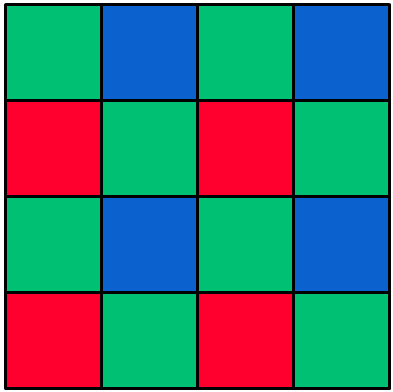
\includegraphics[width=0.3\textwidth]{Bayer1}
\caption{The Bayer pattern image resultant from the bayer filter capture.}
\label{Bayer1}
\end{figure}
 
\begin{figure}[!h]
\centering
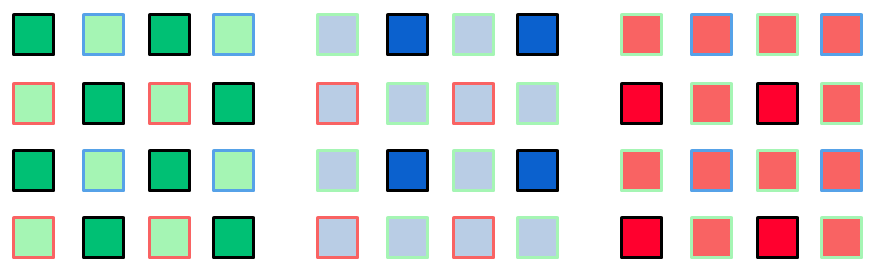
\includegraphics[width=0.9\textwidth]{Bayer2}
\caption{Descriptive diagram of the demosaicking to create the RGB channels from the Bayer pattern image.}
\label{Bayer2}
\end{figure}

The dark boxes in Figure \ref{Bayer2} represent the captured pixel while the lighter boxes are the interpolated locations, with their border showing what color was captured there. Again, there are twice as many green values as blue and red, but all three values are used at their captured spatial locations and then are interpolated to create a three channel RGB image.

Demosaicking is a well-understood and well-researched topic of interest where theories are being developed and applied to improve the interpolation results. The point to grasp here is that color imagery, even before any image processing algorithms are applied, is a sampled, quantized, and interpolated array of data. This shows a significant limitation in the strict accuracy of the initial information within a digital color image. While by no means a crippling factor, understanding this process allows for developing more scientifically stringent arguments for the concessions made later on in the development of the algorithm. For example, given this initial information loss in image capture, multiple-views are developed from statistically (randomly varied) quantized projections of the scene. Parallax and occlusion variations will occur with views at different spatial locations, but this also shows that intensity and color variations will occur in spite of any spatial variation. The views are inherently non-identical in terms of intensity/color, even when capturing the exact same object at the exact same depth and angle. This will be developed further as an important concept of the usefulness of limitations on the metric for the algorithm. There will be many assumptions and simplifications presented as part of the development of this algorithm, and by understanding them as progressing in a foundational manner, starting with those in the imaging system itself, a clear and applicable argument for the choices made in the development of this algorithm will be presented.

Therefore, at this stage, a digital image is seen initially as the demosaicked (interpolated) result of the Bayer pattern image. Stemming from that, a digital image is understood as a rigid, rectangular array of variable bit and channel depth. The number of channels pertains to the color range and the bit depth pertains to the intensity range. Standard contemporary color images are 3-channel (RGB) arrays of the notational size: $\mathfrak{m}\times\mathfrak{n}\times\mathfrak{p}$ (rows-by-columns-by-channels), and have a per pixel bit-depth of 8-bits, resulting in the descriptor of a 24-bit (3-channels with 8-bits each) color image. Variations of these characteristics exist in widespread use, and are important to understand, but the fundamental developments being made here can be easily translated to other image color-types and bit depths, thus all images in the rest of this work will be assumed 8 bits-per-pixel (bpp), 3-channel RGB images. But, the most fundamentally important concept in order to maintain a successful grasp of image processing is the notion that a digital image of size $\mathfrak{m} \times \mathfrak{n} \times \mathfrak{p}$ is akin to a $\mathfrak{p}$-dimensional discrete-space random variable.

Simplifying the discussion to the notion of an $\mathfrak{m} \times \mathfrak{n} \times 1$, henceforth $\mathfrak{m} \times \mathfrak{n}$, image, the functional definition of this image will be: $f(x,y)$. In the image space, $x$ refers to the column-axis and $y$ refers to the row-axis, meaning that the pixel location $(y_{i},x_{j})=(3,4)$ equates to row 3 and column 4, starting from the top left corner of the image (as per the MATLAB\textsuperscript{\textregistered} conventions). Note that $y$ and $x$ are not random vectors, they are independent vectors in either the image (frame) domain in the integer ranges: $[1,\mathfrak{n}]$ and $[1,\mathfrak{m}]$ respectively (again following MATLAB\textsuperscript{\textregistered} notation), or when shown as $\tilde{y}$ and $\tilde{x}$, they are in the global image (scene) domain with continuous ranges: $(-\infty,\infty)$ and $(-\infty,\infty)$. The world function (for the scene) will be denoted as $\tilde{f}(\tilde{x},\tilde{y})$, and is understood as a continuous function of the continuous space. Thus the digital image (a frame from the view of the scene) is known as a projected, sampled, and quantized version of the theoretical real world function (the proposed model of the scene), as mentioned previously. The approximating function's discrete result over the image domain, referred to for simplicity as the intensity image (a random variable), is thus a function of the set of discrete random outcomes of the image capture (the experiment). These terms follow from \cite{Papoulis2002} where the capturing of the light reflected off the scene is understood as the \textbf{experiment}. Each pixel is the projected, sampled, and quantized intensity of that light, and is understood as the \textbf{outcome} of the \textbf{experiment}. Thus the image that is formed can be seen as a function on those intensities and is therefore known as the \textbf{random variable}. The captured image is the two-dimensional (2-D) ($\mathfrak{m}\times\mathfrak{n}$) discrete random variable that is the projected, sampled, and quantized version of the continuous random variable (function) that describes the scene.

Thus as random variables, the images of a scene each have their own Probability Mass Function (PMF) which characterizes them \cite{Papoulis2002}. Though in our discussion we are making the assertion that the Probability Density Function (PDF) that describes the model random variable of the scene is being approximated by the PMF of the image that captures that scene. Each distinct view of the scene should be modeled by a distinct function of the intensities reflected and refracted by the objects in the scene, thus a distinct continuous random variable that will be approximated through image capture by the discrete random variable (image) associated with that view. And so the fundamental assertion being made is that overlapping views should share the same scene model in the overlap. Essentially describing two overlapping views as two random variables with non-trivial conditional probabilities. They are related and can describe each other, in part, because they are captured from the same original model, in that overlap region. And so a joint PMF between two overlapping views will be non-trivial and non-separable, asserting that distinct overlapping views are not independent. This is the foundation for the use of the mutual information metric. Non-mutually exclusive random variables will have some amount of mutual information between them.

And so to finalize the notation and understanding, the discussion is focused on the images captured from the scene. Each view generates an image ($f_{i}$) that is a 2-D random variable over the image domain (from $(1,1)$ to $(\mathfrak{m},\mathfrak{n})$). Each image has come from a projection, sampling, and quantization of the scene at that view that is modeled by $\tilde{f}_{i}$. The scene view has the PDF $\tilde{p}_{i}$ while the image from the view has the PMF $p_{i}$. The rest of the algorithm is built on the registration of two frames, extensible to multiple frames, and so the two images will be described more simply as random variables $A$ and $B$. Thus they will have a joint probability mass of $p_{AB}(\bf{a},\bf{b})$ and their marginal probability masses $p_{A}(\bf{a})$ and $p_{B}(\bf{b})$, where $\bf{a}$ and $\bf{b}$ are the outcomes (the intensities at the pixel locations). The 2-D PMF for digital images is accepted in practice as the normalized intensity histogram. The next section will discuss the relationship between the image histogram and the proposed PMF notation, which will be used to characterize an image (the random variable) and its relationship to the corresponding scene.



%%%%%%%%%%%%%%%%%%%%%%%%%%%%%%%%%%%%%%%%%%%%%%%%%%%%%%%%%%%%%%%%%%%%%%%%%%%%%%%
% END OF DOCUMENT




%************************************
% SECTION 2.3
\section{Histograms and Color Imagery}

\indent
%%%%%%%%%%%%%%%%%%%%%%%%%%%%%%%%%%%%%%%%%%%%%%%%%%%%%%%%%%%%%%%%%%%%%%%%%%%%%%%
%
% Tommy P. Keane
% Master of Science Thesis
% Department of Electrical and Microelectronic Engineering
%
% March 2011
%
%
%
% .tex and .sty modified from:
% http://www.ce.rit.edu/studentresources/gradresource/LaTexThesis.zip
%
%%%%%%%%%%%%%%%%%%%%%%%%%%%%%%%%%%%%%%%%%%%%%%%%%%%%%%%%%%%%%%%%%%%%%%%%%%%%%%%

%%%%%%%%%%%%%%%%%%%%%%%%%%%%%%%%%%%%%%%%%%%%%%%%%%%%%%%%%%%%%%%%%%%%%%%%%%%%%%%
%
% CHAPTER 2
%
% SECTION 3
%
%%%%%%%%%%%%%%%%%%%%%%%%%%%%%%%%%%%%%%%%%%%%%%%%%%%%%%%%%%%%%%%%%%%%%%%%%%%%%%%


%%%%%%%%%%%%%%%%%%%%%%%%%%%%%%%%%%%%%%%%%%%%%%%%%%%%%%%%%%%%%%%%%%%%%%%%%%%%%%%
% BEGIN DOCUMENT

A digital image histogram, referred to by $\textbf{h}(\textbf{n})$, is a discrete function whose dependent variable represents intensity value totals (counted) from the related digital image, and whose independent variable represents the index into the set of sub-ranges (bins) of intensities in the related digital image. The set of intensity values in the range subset is called the bin, having width r, as denoted by Eq. \ref{histBin}. And these independent variables, the range subset indices, are usually used interchangeably with referring to the bin centers. 

\begin{equation}
\label{histBin}
\left[n_{i}-\frac{r}{2},n_{i}+\frac{r}{2}\right)
\end{equation}

Thus, an intensity histogram is a vector holding the sums of intensity values in the sub-ranges. Harkening back to our assumption of images with 8-bits per pixel (8-bpp), this allows for a maximum of 256 unique intensity values per pixel per channel. And again these intensity values are assumed to be statistically random over the 2-D spatial domain of the image. So for a single channel image with 8-bpp a 256 bin histogram can be developed with integer width bins with a total range of $[0,255]$ and sub-ranges (bins): $[n_{i},n_{i+1})$. This histogram is again labeled $\textbf{h}(\textbf{n})$, with $n_{i} \epsilon \{\mathbb{Z}\}_{0}^{256}$, and mathematically the centers can be assumed to be at $\frac{n_{i+1}-n_{i}}{2}$ with width $r=1$, although in practice the half values are outside the 8-bpp intensity range. The total sum of that histogram, as shown in Eq. \ref{histSum}, is the product of the image dimensions, $\mathfrak{m} \cdot \mathfrak{n}$, provided the bins cover the full intensity range. (Note: histograms are defined as a one-to-one transformation of the image data, meaning that no pixel is counted in the histogram more than once)

\begin{equation}
\label{histSum}
	\mathfrak{m} \cdot \mathfrak{n} = \sum_{i=0}^{255}{h(n_{i})}
\end{equation}

As stated, any digital image histogram that covers the entire image and the entire intensity range will always sum to the image size, because all intensity values will fall in the range of the histogram bin intervals, by construction, and can only be counted once, by definition. This is how the PMF can be constructed; by normalizing a histogram by its sum total. The normalization will impose the constraint that an image�s intensity histogram�s sum will equal 1, which is a condition of a PMF; and clearly the histogram describes how many pixels correspond to an intensity value or range, which when normalized can be seen as a corollary to the probability of that intensity value or range occurring within the image. The specificity of the histogram to the image must be recognized though; because what the histogram conveys is that the pixels in \textit{this} image are distributed in \textit{these} amounts. Since an image is a single instance of a random function ($f(x,y)$), and a group of related random functions ($\{f_{1},f_{2},...\}$) should share an equivalent distribution described by their PMF, then a digital image histogram is not identical to a digital PMF, because it is a descriptor of a specific instance of a random function (the image) not a descriptor of the group of functions that this instance originated from. The imaging equivalence made here is that the normalized histogram is cognitively generalized to be a descriptor of the real-world scene that the related image (view�s frame) has captured. This is a very important point of consideration, but its detailed discussion has been deferred to the next section of this chapter and it should be taken for now as an assumption of this development.


After understanding what a histogram is and how to build it, its use is only as good as its limitations. And one of the most important limitations of an intensity histogram is the loss of spatial information in its generation. No spatial information is mathematically present in the calculation of a basic intensity histogram, as it has been described and used herein. However, through basic cognitive information relating to the structure and generation of images, there can be some basic yet significant spatial information extracted from a digital histogram. To illustrate this concept, Figure \ref{sampleHistogram} displays a very simple histogram for a 2-bpp image of size $3\times4$.

\begin{figure}
\label{sampleHistogram}
\centering
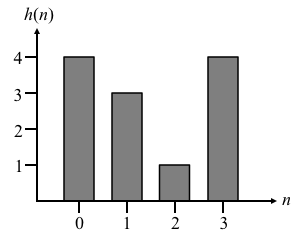
\includegraphics[width=.5\textwidth]{sampleHistogram}
\caption{Example Intensity Histogram}
\end{figure}

What is gathered from this histogram about the image is that there are equal numbers of extreme intensity values, and much more 1s than 2s (here the indices correspond to the intensity values as it is a full-range histogram). This results from a simple reading of the histogram and understanding its basic construction. But in terms of image information, it is also quite clear that this is a mostly dark image with high contrast. This comes from examining the values and structure of the histogram. The values are not bunched up nor are they spread evenly across intensities, so there are some significant edges in the image. Again, though, there is no explicit orientation information present in the mathematical construction of a histogram. Implicitly though this absolutely cannot be a smooth intensity gradient image, meaning that there is no way to construct these pixels with these values so that there is no edge with a transition greater than 1. Figure \ref{sampleImages} shows 4 unique images that all share the histogram shown in Figure \ref{sampleHistogram}.

\begin{figure}
\label{sampleImages}
\centering
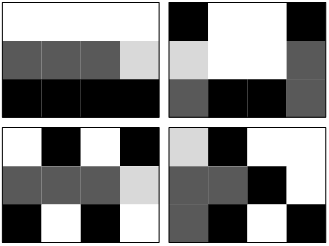
\includegraphics[width=.6\textwidth]{sampleImages}
\caption{Example 2-bpp Images with Identical Intensity Histograms (0 to 3 :: Black to White)}
\end{figure}

After looking at the images in Figure \ref{sampleImages}, the previous assertion becomes clear as there are always several intensity edges of value greater than 1. These images come from the set of 138,600 possible images ($\frac{12!}{4!\cdot4!\cdot3!\cdot1!}$) that share the histogram in Figure \ref{sampleHistogram}. But this is just a mathematical example with no constraints. By the nature of reality, such as the spatial and temporal continuity of objects within reality, images of real scenes are highly constrained subset of all the possible images from the total set (all the possible combinations of intensities given the number of pixels in the image). Any 2-bpp image of size $3\times4$ is actually in a set of $4^{12}$ images, and so the set of images with the histogram in Figure \ref{sampleImages} is roughly less than $0.8\%$ of the total set, while still unconstrained to real world shapes. Thus real world images, constrained by relatively similar histograms, are in an even smaller subset, most likely in the range of $0.05\%$, with a conservative factor of 10 estimate. For example, the images used in this algorithm were all roughly of the size $480 \times 640$ and were 3 channel images of 8-bpp, giving 768 possible values per pixel. This shows that there are $768^{480\cdot640}$ possible images with no spatial or histogram constraint. Any histogram, color constancy model, texture, object contiguity, or any other real world aspect or feature relevant to the digital image will create a smaller and smaller subset. Again, just looking at the previous equation used to calculate the histogram based subset, reapplied in Eq.s \ref{combinatorics} and \ref{bitDepth}, there is a significant decrease in variability.


\begin{equation}
\label{combinatorics}
	\frac{\mathfrak{p} \cdot \left(\mathfrak{m} \cdot \mathfrak{n}\right)!}{ \prod_{i}{\left(n_{i}^{(R)}!\right)} \cdot \prod_{j}{\left(n_{j}^{(G)}!\right)} \cdot \prod_{k}{\left(n_{k}^{(B)}!\right)} }
\end{equation}

\begin{equation}
\label{bitDepth}
	\left( 3 \cdot 2^{b} \right)^{\left(\mathfrak{m} \cdot \mathfrak{n}\right)}
\end{equation}

A rigorous mathematical comparison is not applicable here, but looking at Eq. \ref{combinatorics} compared to Eq. \ref{bitDepth}, it is clear that Eq. \ref{bitDepth} is a monotonically increasing exponential with $\mathfrak{m}$ and $\mathfrak{n}$ while Eq. \ref{combinatorics} is clearly varying with respect to the product of the products in the denominator. The more repetition there is in the given histograms the faster Eq. \ref{combinatorics} will decrease from its already smaller factorial value (compared to the exponential of Eq. \ref{bitDepth}). Again a rigorous discussion is beyond the scope of this work because the purpose here is to illuminate how small the subset of all possible real world images is, and how much smaller the set of all similar images is, and how much smaller the set of similar real world images with similar histograms is. There are several layers of constriction creating such a small subset that clearly the approximation of using a normalized histogram to produce a so-called digital image PDF is a theoretically relevant and a quite realistic simplification. Conceptually what is being stated or assumed is that when viewing the same scene two different views will be essentially sampling the same random function, meaning that they should be describable by the same image PDF. As the overlap decreases between the views the image PDF will be less and less applicable.


This is a direct extension into the WFMI algorithm�s matching scheme and metric calculation. For a large enough image taken from a view that is capturing a scene, there should be enough structure and entropy within the image resultant from the scene (i.e. not just noise) that would allow for another image captured from another view of the scene to share similar data. There will certainly intensity variations, noise concerns, and the data variation coming from occlusion and parallax differences between the views. However, the subsets (regions) of the images that correspond to the same subsets (regions or segments) of the scene should share a similar distribution, or should be accurately conceptually characterized as sharing the same image PDF, in that region. If the images are too small or the region is chosen to be too small, this extension will fail. This can follow mathematically, albeit not presented rigorously here, from Eq.s \ref{combinatorics} and \ref{bitDepth}. As m and n decrease there is less opportunity for variation or consistency in the image, depending upon the value of b. If $2^{b}$ is significant compared to $\mathfrak{m} \cdot \mathfrak{n}$ then each instance of an image from that theoretical set will have significant variation, even when the views are capturing the same scene or sections of the views are capturing the same scene. This is a crippling limit of these assumptions and a source of our empirically derived overlap requirement for the algorithm, as discussed in Chapter 4.


These are extremely important characteristics to understand about intensity histograms. Of course a histogram could be extended to be a spatio-intensity histogram, which would make it a 4-D function with 3 independent variables from the two spatial image axes and the intensity value. But in each channel there is only one pixel at location $\left(0,0\right)$ and that pixel has only one intensity value per channel. The histogram should be seen almost as a projection of the intensity data of the image from the spatial coordinates into a single intensity coordinate. If the spatial information would be considered a full-range spatio-intensity histogram of an m?n?1 image would be the image itself. Significant bin sizes would be needed in the spatial dimensions, but this could be seen as equivalent to finding block-based or region-based histograms, so a definition as such would just be adding unnecessary nomenclature. Also it will be discussed in Chapter 3 as to how computationally taxing the histogram calculation is, and expanding it is a significant detriment to the algorithm. But in considering the assumptions made thus far, note that if spatial information were added into a histogram (especially full-range spatial dependence) the significant occlusions or variations in parallax of the views of the scene would generate very different histograms. Under this scenario, assuming that these different views can be modeled by the same (or in practice, a similar) distribution will be entirely false and misleading. Any image PDF based metric (such as mutual information) will generate a sparse correspondence map because the noise, illumination variations, and scene geometry variations will never align in the same spatial location within the frames from the various views. Avoiding spatial information in the calculation of the image distribution (PDF) is an essential factor in generating a robust algorithm and pushes the results towards conceptual accuracy rather than digital accuracy, as following the model of the trained observer viewing multiple surveillance feeds.


This all follows directly into the generation of, and ambiguities inherent to, mutual information calculations of digital images. So first it is necessary to take a similar look at the calculation of mutual information, and what it can and will represent in this context.


%%%%%%%%%%%%%%%%%%%%%%%%%%%%%%%%%%%%%%%%%%%%%%%%%%%%%%%%%%%%%%%%%%%%%%%%%%%%%%%
% END OF DOCUMENT




%************************************
% SECTION 2.4
\section{Mutual Information}

\indent
%%%%%%%%%%%%%%%%%%%%%%%%%%%%%%%%%%%%%%%%%%%%%%%%%%%%%%%%%%%%%%%%%%%%%%%%%%%%%%%
%
% Tommy P. Keane
% Master of Science Thesis
% Department of Electrical and Microelectronic Engineering
% Rochester Institute of Technology
%
% April 2011
%
%
%
% Funded By: Lenel Systems Inc., A UTC Fire & Security Corporation
%
% Algorithm Intellectual Property Owned By: Lenel Systems Inc.
%
%
% http://www.tommypkeane.com
%
%%%%%%%%%%%%%%%%%%%%%%%%%%%%%%%%%%%%%%%%%%%%%%%%%%%%%%%%%%%%%%%%%%%%%%%%%%%%%%%

%%%%%%%%%%%%%%%%%%%%%%%%%%%%%%%%%%%%%%%%%%%%%%%%%%%%%%%%%%%%%%%%%%%%%%%%%%%%%%%
%
% CHAPTER 2
%
% SECTION 4: Mutual Information
%
%%%%%%%%%%%%%%%%%%%%%%%%%%%%%%%%%%%%%%%%%%%%%%%%%%%%%%%%%%%%%%%%%%%%%%%%%%%%%%%


%%%%%%%%%%%%%%%%%%%%%%%%%%%%%%%%%%%%%%%%%%%%%%%%%%%%%%%%%%%%%%%%%%%%%%%%%%%%%%%
% BEGIN DOCUMENT

To begin, this section will focus on discussing the application of mutual information, which requires a strong understanding of probability and information theory. As was done in Section 2.2 for the probability discussion, there will be some details presented that are necessary for understanding this algorithm and its applications, but most details will be assumed known. Excellent texts to reference for this discussion, pertaining to its development or when in need of a deeper understanding, are \cite{Reza1994}, \cite{MacKay2004}, \cite{Kullback1997}, and \cite{Cover2006}. The text by Cover and Thomas \cite{Cover2006} is an excellent reference for those with an understanding of information theory but are in need of a refresher, while the text by MacKay \cite{MacKay2004} is better suited for those unfamiliar with information theory or the application of probability theory. A lot of the following discussion is best referenced by \cite{Cover2006}.

\begin{figure}[h]
\centering
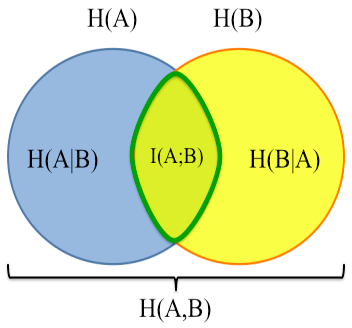
\includegraphics[height=.6\textwidth]{informationTheory}
\caption{Venn diagram of key measures in Information Theory}
\label{informationTheory}
\end{figure}

In a general case, mutual information can be understood as the measurement of the average shared determinism between two random variables; that is, how much does the probability of occurrence of one random variable portray about the probability of occurrence of another. In the case of digital images we are looking at discrete random variables, with their characterizing PMFs (probability of occurrence), and thus discrete entropy measures. Entropy, $H(A)$, is the measure of average randomness in a random variable and is used in the derivation of the mutual information formula. The following information theory terms to be described can be visualized in Figure \ref{informationTheory}. Calculating entropy for the random variable $A$ is shown in Eq. \ref{entropy}. Calculating mutual information in digital images makes it a discrete measure based on discrete random variables and their distributions. Whenever you have two random variables, you can generate a measure of their mutual information, conceptually, by measuring how their marginal entropies relate to their conditional entropy. Again, by referencing Figure \ref{informationTheory}, it is quite clear that there are several ways to determine the mutual information $I(A;B)$. To choose the most appropriate method for calculating mutual information, a view of mutual information applied to image registration can make this derivation much clearer, albeit this is conceptually going in reverse.

\begin{equation}
\label{entropy}
	H(A) = \sum_{i}{p_{A}(a_{i}) \log_{n}{\left(p_{A}(a_{i})\right)}}
\end{equation}

So for the best understanding, this section will start with the digital images and their correspondence, and then work backwards through the registration process to best understand the application of mutual information. In beginning with two digital images, again with an example system image with 8-bpp and a single channel, the question of registration is: what pixels in image A are found in image B? A refinement of this question, thinking more in line with this research, is: what portions or regions, if any, from these images, have captured the same area of the scene? In general, as described in Section 1.2, the four stages of image registration typically deal with pixel correspondences. Once the correspondences are found, the corresponding pixel locations from one image are mapped to their equivalents in the other image, and that mapping is described as an invertible homography. The WFMI algorithm ultimately uses a discrete mutual information measure to determine the correspondences required to register the two images, but it does not look directly for pixel-to-pixel correspondence. The following discussion will present mutual information in terms of its application in this algorithm; a general development is far too rich a topic to cover extensively, so this discussion will begin with entropy measures and their meaning in digital imagery.

Back to the discussion as related to digital imagery, an 8-bpp $\mathfrak{m} \times \mathfrak{n}$ image is a bounded  set of $\mathfrak{m} \cdot \mathfrak{n}$ intensity values distributed randomly in the interval of [0,255]. Corresponding this set to another image, \ie{ }another data set, requires some mathematical measure that is based on mathematical attributes of the data sets themselves, i.e. their PMFs. In Section 2.3 the concept of the intensity histogram was presented and a development for the PMF was presented. Given two digital images, their two intensity histograms can be found, then normalized to generate their image PMFs (also called the marginal PMFs), and then their marginal entropies can be determined through Eq. \ref{entropy}.

Entropy, again, is thought of as the measure of randomness in a random variable, random function, or in this case, a random data set. In communication theory the entropy can be thought of as: the minimum number of bits required to transmit the data over a lossless channel. To translate this understanding to digital imagery, the exact same definition can be used. A digital image is often regarded, generally, as a 3-dimensional function, with digital video being a 4-dimensional function. But given a digital image of size $\mathfrak{m} \times \mathfrak{n} \times \mathfrak{p}$, it can be rearranged to appear as a 1-D signal (a vector, much like a communications signal) of size $(\mathfrak{m} \cdot \mathfrak{n} \cdot \mathfrak{p}) \times 1$. Thus the measure of entropy is presenting the minimum number of bits required to encode or losslessly transmit these $\mathfrak{m} \cdot \mathfrak{n} \cdot \mathfrak{p}$ random pixels. If they are completely random, the entropy is comparably large, but if the data is completely deterministic the entropy approaches 0. The mathematical determination of this randomness measure is essentially characterizing the amount (or lack thereof) of redundancy in the data. This gives a metric of encoding efficiency but not a means of encoding. Therefore it is best to understand entropy as a bounding metric, since it presents the minimum amount of bits for encoding in an ideal situation, which is often not achievable, or in the case of non-integer results, it is not physically possible (i.e. we cannot realistically transmit 3.2 bits, but that is a valid average value). By equations \ref{entropy} and \ref{PMF}, one can take the distribution of a data set and determine its entropy. Classically, $n$ is taken to be 2, so as to create a value $H(A)$ measured as the total number of unique bits required to losslessly encode the data. Equation \ref{PMF} is the equation for generating the image PDF.

\begin{equation}
\label{PMF}
	p_{A}(\bf{a})=h_{A}(\bf{a}) \cdot \left(\sum_{i}{h_{A}(a_{i})} \right)^{-1} = \frac{h_{A}(\bf{a})}{\mathfrak{m}\cdot\mathfrak{n}}
\end{equation}


Now stepping back to the digital image as a data set, it is clear that a measure of entropy can be determined for each image, based on the normalized histograms from Equation \ref{PMF}. Again, since the images are random variables, then joint and conditional probability densities between the images can be determined from joint and conditional histograms. For example, the joint distribution is the normalization of the bivariate intensity histogram. For the bivariate histogram, the $(n_{i},p_{j})${-}bin's value means: there are this many pixels where image A has intensity relating to index $n_{i}$ and image B has intensity relating to index $p_{j}$ at the same spatial location (given images of the same size). In the case of generating the bivariate histogram between an image and itself, the result is an $\mathfrak{m} \times \mathfrak{n}$ ``identity'' matrix since an image will only have a value relating to index $n_{i}$ where itself also has the value relating to index $p_{j}$ when $i \equiv j$. The identity matrix is typically square, but this quoted version means a non-square sparse matrix with diagonal values equal to 1. For example, given $h(0,2)=4$, then what is known is that somewhere in image A there are at least 4 pixels with intensity values in the range of bin 0, and there are at least 4 pixels in image B with intensity values in the range of bin 2, and that only 4 of those pixels in each image are in the exact same spatial locations within the images. That is all that is known and can be extracted from only the bivariate histogram, and so neither image can be rebuilt from the joint histogram, or even with the joint and marginal histograms. At most their spatial contingency upon one another can be determined.

This is a major factor in understanding the application of mutual information, because as is shown in Equation \ref{MutualInformation}, the mutual information is developed from the joint and marginal histograms.

\begin{equation}
\label{MutualInformation}
	I(A,B) = \sum_{j}{\sum_{i}{p_{AB}(a_{i},b_{j}) \log_{2}{\left( \frac{p_{AB}(a_{i},b_{j})}{p_{A}(a_{i})p_{B}(b_{j})}\right)}}}
\end{equation}

\noindent What is immediately apparent is that if the product of the marginal distributions is equal to the joint distribution, then the mutual information is zero. When a joint distribution is equivalent to the product of the marginal distributions the two random variables are said to be independent. So when the random variables are independent, then they will have no mutual information. And again, mutual information is, at its heart, a measure of randomness, i.e. an entropy measure. Joint entropy depicts how random two images are, jointly, by denoting the number of bits required to encode them. Mutual information denotes how much the random information in A can convey knowledge about the random information in B. Thus in the further development of this algorithm the normalized mutual information value presented in Equation \ref{NormalizedMutualInformation} will be used, as developed by the work in \cite{Yao1999} which characterized it as a symmetric and normalized measure.

\begin{equation}
\label{NormalizedMutualInformation}
	I(A,B) = \left( \frac{2}{H(A) + H(B)}\right) \cdot \sum_{j}{\sum_{i}{p_{AB}(a_{i},b_{j}) \log_{2}{\left( \frac{p_{AB}(a_{i},b_{j})}{p_{A}(a_{i})p_{B}(b_{j})}\right)}}}
\end{equation}

\noindent What this provides is a mutual information measure that is dependent only upon the two images, A and B, and their total number of applicable pixels. This will be discussed in more detail in Chapter 3.

What is resultant then is that there is a single value result for any comparison of distributions, with high values meaning similar distributions and values approaching zero (as it is a non-negative measure) meaning dissimilar distributions. Since images or regions of images can be seen as random variables characterized by their distributions, then they too can be compared in this manner. Ultimately the question here will be how to generate the distributions, meaning, what data is used from the images to develop the histograms, and why it is done for these surveillance situations? This will be expanded upon in the discussion of the algorithm in Chapter 3, while the important understanding here is that this is a distribution measure, not an element-by-element measure.


%%%%%%%%%%%%%%%%%%%%%%%%%%%%%%%%%%%%%%%%%%%%%%%%%%%%%%%%%%%%%%%%%%%%%%%%%%%%%%%
% END OF DOCUMENT




%************************************
% SECTION 2.5
\section{Projective Camera Geometry}

\indent
%%%%%%%%%%%%%%%%%%%%%%%%%%%%%%%%%%%%%%%%%%%%%%%%%%%%%%%%%%%%%%%%%%%%%%%%%%%%%%%
%
% Tommy P. Keane
% Master of Science Thesis
% Department of Electrical and Microelectronic Engineering
% Rochester Institute of Technology
%
% April 2011
%
%
%
% Funded By: Lenel Systems Inc., A UTC Fire & Security Corporation
%
% Algorithm Intellectual Property Owned By: Lenel Systems Inc.
%
%
% http://www.tommypkeane.com
%
%%%%%%%%%%%%%%%%%%%%%%%%%%%%%%%%%%%%%%%%%%%%%%%%%%%%%%%%%%%%%%%%%%%%%%%%%%%%%%%

%%%%%%%%%%%%%%%%%%%%%%%%%%%%%%%%%%%%%%%%%%%%%%%%%%%%%%%%%%%%%%%%%%%%%%%%%%%%%%%
%
% CHAPTER 2
%
% SECTION 5: Camera Geometry
%
%%%%%%%%%%%%%%%%%%%%%%%%%%%%%%%%%%%%%%%%%%%%%%%%%%%%%%%%%%%%%%%%%%%%%%%%%%%%%%%


%%%%%%%%%%%%%%%%%%%%%%%%%%%%%%%%%%%%%%%%%%%%%%%%%%%%%%%%%%%%%%%%%%%%%%%%%%%%%%%
% BEGIN DOCUMENT

Sections 2.3 and 2.4 have presented the mathematics and concepts required for building the mutual information metric and applying it to digital images. The final major concept to understand in the theoretical development and motivation is how multiple views of a single scene can be related mathematically. Also, this section presents the major obstacles in multi-view geometry, specifically parallax differences and occlusions, as a mathematical model for relating views is only as useful as its constraints and assumptions when applying it to real-world scenarios.

As the discussion has been already laid out, there are three distinct coordinate systems present in the mathematics discussed here. There are the scene coordinates: the 3-dimensional spatial world with time; the camera (view) coordinates (the digital video): a 2-dimensional spatial domain with a third dimension for color and a fourth dimension for time; and the frame coordinates: the 2-dimensional, plus the third dimension for color, image extracted from the video. The camera view projects the real-world scene onto the 2-D spatial domain of the camera plane while preserving the time dimension (albeit sampled and quantized in all of these dimension), and the frame is an instance of the time dimension of the camera. There is no quantization when looking at the frame versus the video, and it is not conceptually useful to think of it as sampling, it is an extraction. Video compression concerns will be ignored in this development though they play a role in the success of the algorithm, but simplistically they can be thought of as  more quantization and interpolation. Similar to what will be discussed in Chapter 6's review of potential future applications in motion tracking or estimation, multiple frames could be incorporated to build a more accurate metric and alleviate many of the concerns and obstacles of registering multiple views.

Understanding camera geometry is most easily understood by modeling the digital camera as a spatial projection system with a pinhole/point aperture \cite{Hartley2003}. Extending all of the following to realistic apertures would mostly just modify image spatial resolution and essentially creates a blurring effect on the results. Including this would only complicate the discussion as ray geometry would have to be abandoned for wavefront physics. So, again, the camera is thought of as a system that takes the light reflected and refracted off of the objects in the scene, allows it to pass through the point aperture (modeled as rays), and captures the light rays at the sample locations on the CCD array (which again has the Bayer filter in the case of color imagery). Following this understanding of ray optics there will be several main components of the camera model: real-world points, the point/conic/plane at infinity (the vanishing point), the image plane, and the camera center (a point). This model for a single camera is shown in Figure \ref{CameraModel}.

\begin{figure}[h]
\centering
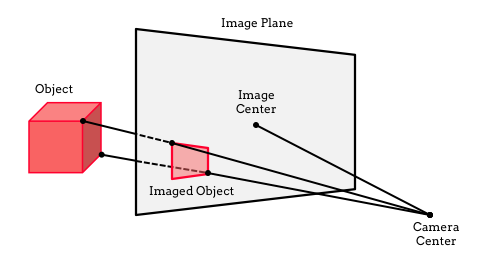
\includegraphics[width=.9\textwidth]{CameraModel}
\caption{Projective Camera System Model}
\label{CameraModel}
\end{figure}


Again, it is clear in this model that there are the 3-D objects in the scene that become projected through the camera aperture (not shown for simplification) onto the camera's image plane as a 2-D imaged object. As the camera center moves in relation to the object in the scene, the projection of the object will clearly change. Looking at Figure \ref{CameraModel}, the idea in this algorithm's applicable scenarios is that the object (the scene) and the cameras (the views) will remain stationary but these other cameras viewing the same object will have distinct projections of the scene onto their image planes. In this model the object is highly symmetric so there will be many views that seem identical but real-world objects are not typically this symmetric; although they do have typically rigid shapes with relatively smooth textures, \ie{ }large areas of low entropy. Clearly for multiple views, the closer the camera centers are, the more similar the views will be. If the scene has many objects and a lot of 3-dimensional spatial variation, then it will require less and less distance between camera centers for the views to change significantly. Yet modeling a general scene as having a significant but not extensive amount of 3-dimensional variation can fall back to the discussion on regional PMFs, where the overlapping regions in the views (the sections of the images observing the same objects in the scene) will be similar enough in intensity or projected scene content that their PMFs should have a higher mutual information than any other combination of regions (in a scene with modest entropy).

But, there are more complex scenarios (that are unfortunately more realistic) where this argument does not seem to follow as directly as it just did. Figure \ref{CameraOcclusion} shows a scene with two objects viewed by two cameras, resulting in the two distinct projections, but now there is clear variation in the amounts of parallax and occlusion in each view's frame.


\begin{figure}[h]
\centering
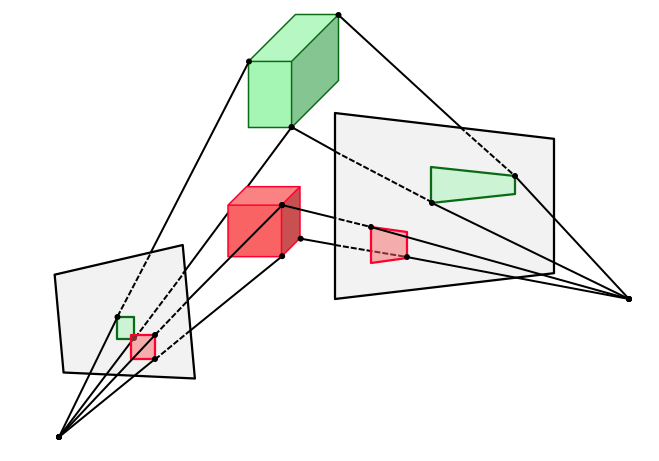
\includegraphics[width=.9\textwidth]{CameraOcclusion}
\caption{Multiple Projective Cameras Model}
\label{CameraOcclusion}
\end{figure}

\noindent The camera on the left's image suffers from occlusion where the red block is covering a corner of the green block, as also indicated by the paths of the rays. There is also the effect of parallax, wherein with each view the distance between projected objects in the images varies based on the camera's distance to the objects in the scene. The red and green blocks appear very close together spatially in the left view but are spaced far apart in the right view. Occlusion and parallax are not just characteristics of the views, they are characteristic of the entire scenario: the scene, its objects, and the views. This model, however, is an extreme case as a panorama would not be easily generated or viewable in a 2-D display given these views. Also, the objects imaged are essentially being imaged orthogonally by the cameras and so without some strong symmetry in the objects there would be no correspondence between the views; and that symmetry would be a false registration, just as in the case of registering two non-overlapping views of an extremely low entropy scene (constant colored or textured flat surface). The registration could seem accurate but it would be trivial and incorrect, which would be discernible as soon as an object began a non-symmetrical motion (that is symmetry between the views).

So ultimately what is applicable to this algorithm that needs to be understood about camera geometry? Projection is the main thrust of this discussion, even though multi-view geometry is an extremely rich and interesting topic, because the goal of this algorithm is to generate convincing panoramas of realistic scenes, automatically. Views like those modeled in Figure \ref{CameraOcclusion} are certainly relatable through epipolar constraints and use of a Fundamental matrix \cite{Hartley2003}, but they would not produce a 2-D panorama. Clearly there must be some initial restriction, in the basic theory, where camera centers are not at angles of rotation much beyond 45\textsuperscript{o} to one another with respect to their views. Realistically, \ie{ }in practice, this is a general and typical scenario as cameras will be placed along typically rectangular structures such as buildings and fence lines or in hallways. Yet even in these scenarios, there will be significant occurrences of occlusion, and differences in occlusion between views stemming from parallax discrepancies. If an object is occluded in one view and not the other, such as the bottom corner of the green box, any point-to-point correspondence algorithm that considered that corner of the box a feature, would find it in one view but not the other, thus that correspondence would not and could not be used in registration. The more complex the scene is, such as irregular shaped objects and large variations in 3-dimensional arrangements, there will be many points existing in one view that do not exist in the other. This discussion will be expanded in the next chapter, but this is the foundational motivation for designing the WFMI algorithm as a region-based correspondence rather than a point-based correspondence algorithm. And limiting it to rigid contiguous regions maintains the structure of the scene. Point-to-point correspondence can allow for more realistic deformations, but it can also allow for very unrealistic deformations. Given that that corner of the green box was found in one view and not the other, it could be searched for in the second view and accidentally corresponded to some other point in the scene. Using that relationship to develop the homography or transformation between the views \cite{Hartley2003} can produce extreme inaccuracy.

The next chapter will discuss the details of the implementation of the algorithm based on these theories, but it is important to understand that occlusion and parallax are extremely difficult to model but occur extremely often in realistic scenarios. With no known relationship between camera locations, the WFMI algorithm took this knowledge of multi-view geometry and its constraints to assume that even though there will not be a full set of points in an overlap region that can be corresponded, the structure and arrangement of objects will be there and that's what should be searched for. This is why it is a region based algorithm, as it compares scenes based on the structure and arrangement of the objects, not the exact location of the objects. That is also why it is so successful despite only searching for an affine relationship between views more accurately relatable by a projective homography or a Fundamental matrix.

%%%%%%%%%%%%%%%%%%%%%%%%%%%%%%%%%%%%%%%%%%%%%%%%%%%%%%%%%%%%%%%%%%%%%%%%%%%%%%%
% END OF DOCUMENT







%%%%%%%%%%%%%%%%%%%%%%%%%%%%%%%%%%%%%%%%%%%%%%%%%%%%%%%%%%%%%%%%%%%%%%%%%%%%%%%
% CHAPTER 3
\chapter{Algorithm}

\indent
%%%%%%%%%%%%%%%%%%%%%%%%%%%%%%%%%%%%%%%%%%%%%%%%%%%%%%%%%%%%%%%%%%%%%%%%%%%%%%%
%
% Tommy P. Keane
% Master of Science Thesis
% Department of Electrical and Microelectronic Engineering
% Rochester Institute of Technology
%
% April 2011
%
%
%
% Funded By: Lenel Systems Inc., A UTC Fire & Security Corporation
%
% Algorithm Intellectual Property Owned By: Lenel Systems Inc.
%
%
% http://www.tommypkeane.com
%
%%%%%%%%%%%%%%%%%%%%%%%%%%%%%%%%%%%%%%%%%%%%%%%%%%%%%%%%%%%%%%%%%%%%%%%%%%%%%%%

%%%%%%%%%%%%%%%%%%%%%%%%%%%%%%%%%%%%%%%%%%%%%%%%%%%%%%%%%%%%%%%%%%%%%%%%%%%%%%%
%
% CHAPTER 3
%
% PREAMBLE: The Algorithm and Implementation
%
%%%%%%%%%%%%%%%%%%%%%%%%%%%%%%%%%%%%%%%%%%%%%%%%%%%%%%%%%%%%%%%%%%%%%%%%%%%%%%%


%%%%%%%%%%%%%%%%%%%%%%%%%%%%%%%%%%%%%%%%%%%%%%%%%%%%%%%%%%%%%%%%%%%%%%%%%%%%%%%
% BEGIN DOCUMENT

With a robust understanding of the foundational mathematics and concepts, the discussion of the algorithm focuses on understanding the practicalities that molded the application of the theory. Limitations and the success of the results will be discussed in Chapter 5 with the results themselves. The first section of this chapter will break down the major components of the algorithm into subsections, focusing on the implementation details while drawing from the foundational mathematics discussed in the previous chapter. The second section will then take a ``big picture'' overview of the algorithm, discussing how the components from those previous subsections all come together to form the fully functional algorithm. This allows a first-time reader to work from the nuts-and-bolts up to the big picture, while also providing a researcher the opportunity to skip to section 2 for a review of the algorithm and its applied models. This chapter will also discuss the process of the actual implementation of the algorithm in MATLAB\textsuperscript{\textregistered} and OpenCV alongside the details of the implementation.



%%%%%%%%%%%%%%%%%%%%%%%%%%%%%%%%%%%%%%%%%%%%%%%%%%%%%%%%%%%%%%%%%%%%%%%%%%%%%%%
% END OF DOCUMENT



%************************************
% SECTION 3.1
\section{Algorithm Components}

\indent
%%%%%%%%%%%%%%%%%%%%%%%%%%%%%%%%%%%%%%%%%%%%%%%%%%%%%%%%%%%%%%%%%%%%%%%%%%%%%%%
%
% Tommy P. Keane
% Master of Science Thesis
% Department of Electrical and Microelectronic Engineering
% Rochester Institute of Technology
%
% May 2011
%
%
% Funded By: Lenel Systems Inc., A UTC Fire & Security Corporation
%
% Algorithm Intellectual Property Owned By: Lenel Systems Inc.
%
%
% http://www.tommypkeane.com
%
%%%%%%%%%%%%%%%%%%%%%%%%%%%%%%%%%%%%%%%%%%%%%%%%%%%%%%%%%%%%%%%%%%%%%%%%%%%%%%%

%%%%%%%%%%%%%%%%%%%%%%%%%%%%%%%%%%%%%%%%%%%%%%%%%%%%%%%%%%%%%%%%%%%%%%%%%%%%%%%
%
% CHAPTER 3
%
% SECTION 1: Algorithm Components
%
%%%%%%%%%%%%%%%%%%%%%%%%%%%%%%%%%%%%%%%%%%%%%%%%%%%%%%%%%%%%%%%%%%%%%%%%%%%%%%%


%%%%%%%%%%%%%%%%%%%%%%%%%%%%%%%%%%%%%%%%%%%%%%%%%%%%%%%%%%%%%%%%%%%%%%%%%%%%%%%
% BEGIN DOCUMENT

The basic algorithm contains 5 major steps as shown in the flowchart in Figure \ref{algorithmFlowchart} below. This chart shows the processing order of each step, but purposefully has labeled them by their goal and not their specific implementation details. The exact processes of the algorithm will be explained in the following subsections, but, as is the intended purpose of the flowchart, it should be kept in mind that the specific operations were chosen to serve the goals. The overall algorithm itself could be implemented differently as long as the main goals in each step are met. This will be discussed further in Chapter 5 as a possibility for future work in modifying some of the chosen means of implementing these components. The story of the development of the implementation is presented alongside the purpose and method of implementation, as they are interrelated.

\begin{figure}
\centering
\vskip-.25in
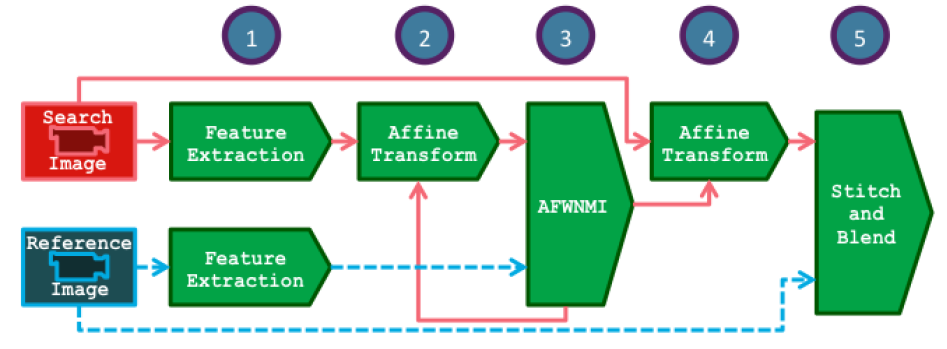
\includegraphics[width=.95\textwidth]{flowchartHorizontal}
\caption{Algorithm Flowchart}
\label{algorithmFlowchart}
\end{figure}


%%%%%%%%%%%%%%%%%%%%%%%%%%%%%%%%%%%%%%%%%%%%%%%%%%%%%%%%%%%%%%%%%%%%%%%%%%%%%%%
% END OF DOCUMENT



%************************************
% SECTION 3.1.1
\subsection{Feature Extraction}

\indent
%%%%%%%%%%%%%%%%%%%%%%%%%%%%%%%%%%%%%%%%%%%%%%%%%%%%%%%%%%%%%%%%%%%%%%%%%%%%%%%
%
% Tommy P. Keane
% Master of Science Thesis
% Department of Electrical and Microelectronic Engineering
% Rochester Institute of Technology
%
% April 2011
%
%
%
% Funded By: Lenel Systems Inc., A UTC Fire & Security Corporation
%
% Algorithm Intellectual Property Owned By: Lenel Systems Inc.
%
%
% http://www.tommypkeane.com
%
%%%%%%%%%%%%%%%%%%%%%%%%%%%%%%%%%%%%%%%%%%%%%%%%%%%%%%%%%%%%%%%%%%%%%%%%%%%%%%%

%%%%%%%%%%%%%%%%%%%%%%%%%%%%%%%%%%%%%%%%%%%%%%%%%%%%%%%%%%%%%%%%%%%%%%%%%%%%%%%
%
% CHAPTER 3
%
% SECTION 1.1: Feature Extraction
%
%%%%%%%%%%%%%%%%%%%%%%%%%%%%%%%%%%%%%%%%%%%%%%%%%%%%%%%%%%%%%%%%%%%%%%%%%%%%%%%


%%%%%%%%%%%%%%%%%%%%%%%%%%%%%%%%%%%%%%%%%%%%%%%%%%%%%%%%%%%%%%%%%%%%%%%%%%%%%%%
% BEGIN DOCUMENT

For the WFMI algorithm it was reasoned that the initial stage of feature extraction should be simple enough to allow the eventual possibility of real-time operation, but must still provide robust enough features to secure success in a variety of complex and unknown scenarios. Looking to the work in \cite{Ugarriza2009} the choice of color gradient features was found appropriate to provide a robust set of non-rigid shape details that, even under scaling and quantization, preserve a significant amount of the original information from the color video frames. After generating the RGB-gradient map (which is a floating point single channel image) a quantization step was implemented to achieve a computationally efficient algorithm.

Given an $\mathfrak{m}\times\mathfrak{n}$ 8-bpp pair of 3-channel color images, each  image (typically $480\times640$) is first processed to extract a feature map. The algorithm from \cite{Lee1991} is a vector-space gradient operation calculated by using the vectorized color pixel values ($\mathfrak{p}\times1$ vectors) as locations in the current color space (\ie RGB in this implementation). Taking horizontal and vertical gradients along each channel in the intensity domain and then using those resultant gradient images as inputs to the calculation of the maximum eigenvalue of the color-space Jacobian provides an essentially infinite, floating-point range of intensity values in the resultant color gradient map (again: single channel). In a practical implementation, there is an earlier, intial quantization required to limit this theoretically infinite floating-point map to the bit-depth of data-type. In the MATLAB\textsuperscript{\textregistered} and OpenCV implementations this was set to 64-bits, and this is the maximum amount of information that can be generated or stored by these features. Any quantization operation beyond this will superfluously remove information, but will enhance computational efficiency in the PMF calculation which has a range of $2^{b}$ (with $b$ being the bit-depth) maximum bins; so the key is to then discern what amount of quantization will maintain enough information to generate an appropriate and accurate mutual information map that is applicable for further processing in the registration search.

In order to determine the appropriate amount of quantization it is necessary to look ahead to the next step of the algorithm. The subsequent step of the algorithm is to perform an affine transform search with an exhaustive translation search. This will be explained in Section 3.1.2, but in order to perform a computationally efficient search with a metric based on joint and marginal PMF calculations for each translation in the exhaustive search, there is a need to quantize the color gradient maps into the ``edge'' maps. This secondary quantization results in maps on the order of one to four bits of pixel depth (still single channel) thus providing on the order of 3 to 30 distinct ``edges''. Since the PMF calculations will be based on full range histograms, as was discussed, then the joint PMF size will be $2^{b_{e}}\cdot2^{b_{e}}$, where $b_{e}$ is the bit-depth of the gradient to ``edge'' quantization. (Note: the use of ``edge'' is to maintain that this is not a binary map, there is no thresholding operation, the gradient is simply quantized so a syntactical distinction is being made.)

The stronger the quantization, \ie{ }the fewer the number of ``edges'', the less information available in the image from the color-space gradient map, yet this is inversely proportional to the computational efficiency. Also, discussed in more detail later on, in the use of a hierarchical search there is an added concern as to the effects of the subsampling on the image information. These are all significant implementation concerns, and it was found that the fastest and most accurate implementation was achieved with $b_{e}=2$, thus having 4 significant ``edges'' while zero values were ignored in the PMF calculations. To determine the quantization a simplification of the method in \cite{Ugarriza2009} was used where the gradient map histogram was quantized. The top 20\% of the pixels were empirically determined as the strong object ``edges'', with the bottom 10\% being determined as noise or superfluous detail ``edges''. The remaining 70\% of the pixels were evenly split into $b_{e}-1$ groups of so-called significant detail ``edges''. As the gradient histogram was found to typically follow a low-variance poission-like distribution with right skew, these percentage bounds were found to empirically average the distribution rise with the bottom 10\%, the long tail with the top 20\%, and the majority of the distribution with the middle 70\%. This was an empirical development that is fast, efficient, and has been found to provide useful and conceptually valid ``edges'' in the realistic test images. A visualization of this quantization is shown in Figure \ref{gradienthistogram}.

\begin{figure}[h]
\centering
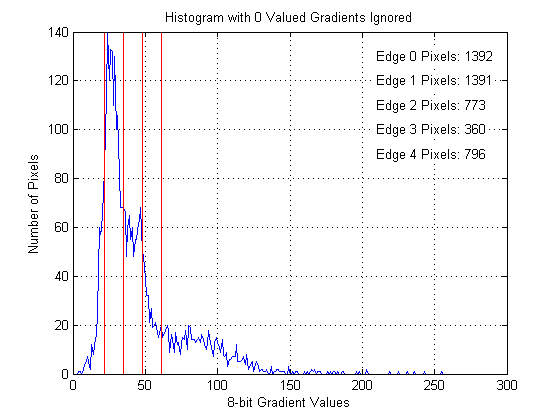
\includegraphics[width=.8\textwidth]{GradientHistogram}
\caption{Example Gradient Map Histogram with Quantization Boundaries}
\label{gradienthistogram}
\end{figure}


%%%%%%%%%%%%%%%%%%%%%%%%%%%%%%%%%%%%%%%%%%%%%%%%%%%%%%%%%%%%%%%%%%%%%%%%%%%%%%%
% END OF DOCUMENT



%************************************
% SECTION 3.1.2
\subsection{Affine Transform Search}

\indent
%%%%%%%%%%%%%%%%%%%%%%%%%%%%%%%%%%%%%%%%%%%%%%%%%%%%%%%%%%%%%%%%%%%%%%%%%%%%%%%
%
% Tommy P. Keane
% Master of Science Thesis
% Department of Electrical and Microelectronic Engineering
% Rochester Institute of Technology
%
% April 2011
%
%
%
% Funded By: Lenel Systems Inc., A UTC Fire & Security Corporation
%
% Algorithm Intellectual Property Owned By: Lenel Systems Inc.
%
%
% http://www.tommypkeane.com
%
%%%%%%%%%%%%%%%%%%%%%%%%%%%%%%%%%%%%%%%%%%%%%%%%%%%%%%%%%%%%%%%%%%%%%%%%%%%%%%%

%%%%%%%%%%%%%%%%%%%%%%%%%%%%%%%%%%%%%%%%%%%%%%%%%%%%%%%%%%%%%%%%%%%%%%%%%%%%%%%
%
% CHAPTER 3
%
% SECTION 1.2: Affine Transform Search
%
%%%%%%%%%%%%%%%%%%%%%%%%%%%%%%%%%%%%%%%%%%%%%%%%%%%%%%%%%%%%%%%%%%%%%%%%%%%%%%%


%%%%%%%%%%%%%%%%%%%%%%%%%%%%%%%%%%%%%%%%%%%%%%%%%%%%%%%%%%%%%%%%%%%%%%%%%%%%%%%
% BEGIN DOCUMENT

The affine transformation is defined by 4 distinct operations: scale, skew, rotation, and translation. Skew, translation, and scale can each be defined separately for the rows and for the columns of the image. This allows for more complex deformations but from the understanding of projective geometry, it would be more accurate to model realistic deformations by different amounts of scaling or skew variation across the view, not just a constant transformation equally along all the rows versus another equally across all the columns. This approach was not investigated because the current implementation of the algorithm already performs an exhaustive translation search and research into more complex transformations proved to unacceptably increase computation costs.

The most drastic assumption made by the WFMI algorithm is in the utilization of an affine-only search for image registration in views with relationships significantly outside affine constraints. This was an assumption made mostly for computational efficiency and simplicity, it is not an assumption based on a strong mathematical or conceptual understanding such as the assumptions discussed in Chapter 2. That being said, it is an efficient and robust means of generating estimates for accurate registration between overlapping views of complex scenes. In the actual implementation the affine transform was not usually implemented but a similarity transform (rotation, scale, and translation only) was used instead. It was found that in most scenarios, skew had little to no effect on providing a more convincing view and so that dimension of the search space was ignored. That is in practice only; in the design of the algorithm it is part of the full implementation. It was also found that between rotation and scaling, rotation proved the more important factor in creating a convincing view. The reasons behind this will be discussed with the results presented in Chapter 4, as the rest of the algorithm must be explored first.

The affine (or similarity) transform search has been implemented in practice as a limited search in rotation, scale, and skew, with an exhaustive translation search. While it is maintained that this is a fully automatic algorithm, there is the practical consideration that between two overlapping views of a realistic scene there will not be views rotated by 90\textsuperscript{o} between them or scaled by 100\%. With that understanding, then, it was found through testing that realistic scenes with average overlap (usually 20-40\%) were in the range of $-15^{o}$ to $15^{o}$ of rotation and a scale factor of $0.8$ to $1.2$ was a generous range. While skew was usually ignored in the actual implementation, it can be an overcompensating factor and so while a range similar to the scale factor seems reasonable, it was usually restricted to about half that range, to maintain more reasonable results. The main problem with skew is that when deforming an entire image, it did not prove to be a reliable estimate for the effects of parallax and projective distortion in views of realistic scenes. Again, more of the algorithm needs to be discussed first, so this will be elaborated on in the following chapter, but skew tended to promote mis-registration of low entropy regions as it allows the view to distort in an unrealistic manner.

The search itself is done as two stages. First, one image is chosen as the reference image; the affine homography to be found will be a transformation for the second image (the search image) onto this first image (the reference image). The homography should be invertible and so the reference image could be transformed onto the search image using the inverse of the transform matrix, but this is more of a mathematical consideration than a practical one \cite{Hartley2003}. In the case of a full affine search, the skew, scale, and rotation ranges are pre-defined (as was mentioned, this is a practical limitation) and the search space is the three-dimensional space covered by these ranges. At this point translation is being ignored. Once the reference image (following the left path of Figure \ref{algorithmFlowchart}) is chosen and the affine (without translation) search space is defined, the second image (following the right path of Figure \ref{algorithmFlowchart}) undergoes a transformation in this space. For this implementation there was no enhancement made to the navigation of the search space and so the skew-scale-rotation-space (affine search space) is searched linearly, which may not be the most accurate method. Once the second image has undergone the transformation it is now a temporary new image and it is passed to the correspondence stage (Section 3.1.3) along with the unmodified reference image for comparison. Note, this is done at the top level of the Gaussian pyramid created for the hierarchical search, and this is done on the 64-bit color gradient image maps.

The flowchart of Figure \ref{algorithmFlowchart} is conceptually accurate but in practice, especially during the transition from MATLAB\textsuperscript{\textregistered} to OpenCV, it was found that the Gaussian pyramid reduction adds superfluous quantization to the ``edge'' images. This was found in the OpenCV implementation because C++ is a hard-typed language and MATLAB\textsuperscript{\textregistered} defaults to 64-bit data; so in the prototyping stage it was not initially recognized that the $b_{e}$-bit ``edge'' images were actually being stored as 64-bit images. What this requires then is to first build the Gaussian pyramid with the 64-bit gradient maps, choose the reference and search images, transform the search gradient map, and once it is transformed it can quantized into the $b_{e}$-bit ``edge'' map. After choosing the reference image, it can be quantized as well. The correspondence stage (Section 3.1.3) is thus working on the reference image's ``edge'' map and the transformed search image's ``edge'' map, which are from the top of the Gaussian pyramid for the hierarchical search. In both implementations these images are padded with zero values (since zero is ignored as data) to be the same size.

The next section will discuss the implementation of translation, but a final remark is to note that in the overview of the algorithm it is important to keep in mind that the correspondence is occurring in the skew-scale-rotation-space. So for every combination of skew, scale, and rotation (every point in that discrete 3-D space) a peak from the filtered and weighted mutual information map will be found and will be compared to the rest of the space. In implementation, to save memory, each time the temporary image is created by the transformation of the search image, it is replaced when moving to the next transformation in the affine search space. In Figure \ref{algorithmFlowchart} there is a second transformation after the WFMI stage (the correspondence search), and this second transformation is defining the final transformation for the search image based on the results from the correspondence search. Again, since each transformation was thrown out during the search, once the optimal peak is found from the affine search, the corresponding affine transform must be reapplied to the search image, while the reference image still remains unmodified.

%%%%%%%%%%%%%%%%%%%%%%%%%%%%%%%%%%%%%%%%%%%%%%%%%%%%%%%%%%%%%%%%%%%%%%%%%%%%%%%
% END OF DOCUMENT




%************************************
% SECTION 3.1.3
\subsection{Weighted and Filtered Mutual Information}

\indent
%%%%%%%%%%%%%%%%%%%%%%%%%%%%%%%%%%%%%%%%%%%%%%%%%%%%%%%%%%%%%%%%%%%%%%%%%%%%%%%
%
% Tommy P. Keane
% Master of Science Thesis
% Department of Electrical and Microelectronic Engineering
%
% March 2011
%
%
%
% .tex and .sty modified from:
% http://www.ce.rit.edu/studentresources/gradresource/LaTexThesis.zip
%
%%%%%%%%%%%%%%%%%%%%%%%%%%%%%%%%%%%%%%%%%%%%%%%%%%%%%%%%%%%%%%%%%%%%%%%%%%%%%%%

%%%%%%%%%%%%%%%%%%%%%%%%%%%%%%%%%%%%%%%%%%%%%%%%%%%%%%%%%%%%%%%%%%%%%%%%%%%%%%%
%
% CHAPTER 3
%
% SECTION 1.3
%
%%%%%%%%%%%%%%%%%%%%%%%%%%%%%%%%%%%%%%%%%%%%%%%%%%%%%%%%%%%%%%%%%%%%%%%%%%%%%%%


%%%%%%%%%%%%%%%%%%%%%%%%%%%%%%%%%%%%%%%%%%%%%%%%%%%%%%%%%%%%%%%%%%%%%%%%%%%%%%%
% BEGIN DOCUMENT

Up to this point the discussion of mutual information has described it as a measure based on random variables. Those random variables were then attributed to the sets of feature values in digital images. Thus making mutual information a mapped measurement, meaning that with two digital images and their set of features mapped in the respective image spaces, the mutual information could be found between overlapping sets of features as the images are put through various spatial transformations. By applying a non-translational affine transformation (i.e. a combination of skewing, scaling, and rotation) the images can be put through a brute force translation search that creates a mutual information measurement for each translation, since each translation provides a new overlap region with the feature images.

Map size $M \times N = (2\mathfrak{m}-1) \times (2\mathfrak{n}-1)$

\begin{equation}
\label{WeightedInformation}
	I_{w}(A,B)=w(A,B) \cdot I(A,B)
\end{equation}


\begin{equation}
\label{}
w(A,B)=\sum_{j}\sum_{i}{h_{A}(a_{i})h_{B}(b_{j})}
\end{equation}


\begin{equation}
\label{}
A_{u}=\{x,y\}_{u} \rightarrow \left\{ \mathcal{O}_{T}\left(\mathcal{A}(x,y) \right) \right\}_{u} 
\end{equation}


\begin{equation}
\label{}
B_{v}=\{x,y\}_{v} \rightarrow \left\{ \mathcal{O}_{T}\left(\mathcal{A}(x,y) \right) \right\}_{v}
\end{equation}


\begin{equation}
\label{}
\mathfrak{w}(A,B)=\sum_{j}\sum_{i}{h_{A_{u}}(a_{i})h_{B_{v}}(b_{j})}
\end{equation}

\begin{equation}
\label{}
\mathfrak{I}(u,v)=I(A_{u},B_{v})=\left(\frac{2}{H(A_{u})+H(B_{v})}\right)
\end{equation}


\begin{equation}
\label{WeightedInformation}
	\mathfrak{I}_{\mathfrak{w}}(u,v)=\mathfrak{w}(u,v) \cdot \mathfrak{I}(u,v)
\end{equation}


\begin{equation}
\label{laplacianFilter}
	L(u,v)=\frac{4}{(\alpha + 1)} \cdot
	\begin{bmatrix}
		\frac{\alpha}{4} & \frac{(1-\alpha)}{4} & \frac{\alpha}{4} \\
		\frac{(1-\alpha)}{4} & -1 & \frac{(1-\alpha)}{4} \\
		\frac{\alpha}{4} & \frac{(1-\alpha)}{4} & \frac{\alpha}{4}
	\end{bmatrix}, \quad \alpha \in [0,1)
\end{equation}

\begin{equation}
\label{FilteredWeightedInformation}
	\mathfrak{I}_{L\mathfrak{w}}(u,v)=L(u,v) \ast \mathfrak{I}_{\mathfrak{w}}(u,v)
\end{equation}

\begin{equation}
\label{peakLocation}
	(\delta_{x},\delta_{y})=\max_{u,v}\left(\mathfrak{I}_{L\mathfrak{w}}\right)
\end{equation}

\begin{equation}
\label{peakTranslation}
	(t_{x},t_{y})=(k,l) \cdot \left| (\delta_{x},\delta_{y}) - (M,N) \right|
\end{equation}

\begin{equation}
\label{peakTranslation}
	[k,l] = \left[ \left| (\delta_{x},\delta_{y}) - (M,N) \right| \le (M,N) \right] - [1,1]
\end{equation}

From the vector Equation \ref{peakTranslation}, $k$ and $l$ will be either $-1$ or $1$.


%%%%%%%%%%%%%%%%%%%%%%%%%%%%%%%%%%%%%%%%%%%%%%%%%%%%%%%%%%%%%%%%%%%%%%%%%%%%%%%
% END OF DOCUMENT




%************************************
% SECTION 3.1.4
\subsection{Affine Homography}

\indent
%%%%%%%%%%%%%%%%%%%%%%%%%%%%%%%%%%%%%%%%%%%%%%%%%%%%%%%%%%%%%%%%%%%%%%%%%%%%%%%
%
% Tommy P. Keane
% Master of Science Thesis
% Department of Electrical and Microelectronic Engineering
% Rochester Institute of Technology
%
% April 2011
%
%
%
% Funded By: Lenel Systems Inc., A UTC Fire & Security Corporation
%
% Algorithm Intellectual Property Owned By: Lenel Systems Inc.
%
%
% http://www.tommypkeane.com
%
%%%%%%%%%%%%%%%%%%%%%%%%%%%%%%%%%%%%%%%%%%%%%%%%%%%%%%%%%%%%%%%%%%%%%%%%%%%%%%%

%%%%%%%%%%%%%%%%%%%%%%%%%%%%%%%%%%%%%%%%%%%%%%%%%%%%%%%%%%%%%%%%%%%%%%%%%%%%%%%
%
% CHAPTER 3
%
% SECTION 1.4
%
%%%%%%%%%%%%%%%%%%%%%%%%%%%%%%%%%%%%%%%%%%%%%%%%%%%%%%%%%%%%%%%%%%%%%%%%%%%%%%%


%%%%%%%%%%%%%%%%%%%%%%%%%%%%%%%%%%%%%%%%%%%%%%%%%%%%%%%%%%%%%%%%%%%%%%%%%%%%%%%
% BEGIN DOCUMENT

TO BE WRITTEN


%%%%%%%%%%%%%%%%%%%%%%%%%%%%%%%%%%%%%%%%%%%%%%%%%%%%%%%%%%%%%%%%%%%%%%%%%%%%%%%
% END OF DOCUMENT




%************************************
% SECTION 3.1.5
\subsection{Stitching and Blending}

\indent
%%%%%%%%%%%%%%%%%%%%%%%%%%%%%%%%%%%%%%%%%%%%%%%%%%%%%%%%%%%%%%%%%%%%%%%%%%%%%%%
%
% Tommy P. Keane
% Master of Science Thesis
% Department of Electrical and Microelectronic Engineering
% Rochester Institute of Technology
%
% April 2011
%
%
%
% Funded By: Lenel Systems Inc., A UTC Fire & Security Corporation
%
% Algorithm Intellectual Property Owned By: Lenel Systems Inc.
%
%
% http://www.tommypkeane.com
%
%%%%%%%%%%%%%%%%%%%%%%%%%%%%%%%%%%%%%%%%%%%%%%%%%%%%%%%%%%%%%%%%%%%%%%%%%%%%%%%

%%%%%%%%%%%%%%%%%%%%%%%%%%%%%%%%%%%%%%%%%%%%%%%%%%%%%%%%%%%%%%%%%%%%%%%%%%%%%%%
%
% CHAPTER 3
%
% SECTION 1.3
%
%%%%%%%%%%%%%%%%%%%%%%%%%%%%%%%%%%%%%%%%%%%%%%%%%%%%%%%%%%%%%%%%%%%%%%%%%%%%%%%


%%%%%%%%%%%%%%%%%%%%%%%%%%%%%%%%%%%%%%%%%%%%%%%%%%%%%%%%%%%%%%%%%%%%%%%%%%%%%%%
% BEGIN DOCUMENT

TO BE WRITTEN


%%%%%%%%%%%%%%%%%%%%%%%%%%%%%%%%%%%%%%%%%%%%%%%%%%%%%%%%%%%%%%%%%%%%%%%%%%%%%%%
% END OF DOCUMENT




%************************************
% SECTION 3.2
\section{Algorithm Overview}

\indent
%%%%%%%%%%%%%%%%%%%%%%%%%%%%%%%%%%%%%%%%%%%%%%%%%%%%%%%%%%%%%%%%%%%%%%%%%%%%%%%
%
% Tommy P. Keane
% Master of Science Thesis
% Department of Electrical and Microelectronic Engineering
%
% March 2011
%
%
%
% .tex and .sty modified from:
% http://www.ce.rit.edu/studentresources/gradresource/LaTexThesis.zip
%
%%%%%%%%%%%%%%%%%%%%%%%%%%%%%%%%%%%%%%%%%%%%%%%%%%%%%%%%%%%%%%%%%%%%%%%%%%%%%%%

%%%%%%%%%%%%%%%%%%%%%%%%%%%%%%%%%%%%%%%%%%%%%%%%%%%%%%%%%%%%%%%%%%%%%%%%%%%%%%%
%
% CHAPTER 3
%
% SECTION 2
%
%%%%%%%%%%%%%%%%%%%%%%%%%%%%%%%%%%%%%%%%%%%%%%%%%%%%%%%%%%%%%%%%%%%%%%%%%%%%%%%


%%%%%%%%%%%%%%%%%%%%%%%%%%%%%%%%%%%%%%%%%%%%%%%%%%%%%%%%%%%%%%%%%%%%%%%%%%%%%%%
% BEGIN DOCUMENT

TO BE WRITTEN


%%%%%%%%%%%%%%%%%%%%%%%%%%%%%%%%%%%%%%%%%%%%%%%%%%%%%%%%%%%%%%%%%%%%%%%%%%%%%%%
% END OF DOCUMENT





%%%%%%%%%%%%%%%%%%%%%%%%%%%%%%%%%%%%%%%%%%%%%%%%%%%%%%%%%%%%%%%%%%%%%%%%%%%%%%%
% CHAPTER 4
\chapter{Results}

\indent
%%%%%%%%%%%%%%%%%%%%%%%%%%%%%%%%%%%%%%%%%%%%%%%%%%%%%%%%%%%%%%%%%%%%%%%%%%%%%%%
%
% Tommy P. Keane
% Master of Science Thesis
% Department of Electrical and Microelectronic Engineering
% Rochester Institute of Technology
%
% April 2011
%
%
%
% Funded By: Lenel Systems Inc., A UTC Fire & Security Corporation
%
% Algorithm Intellectual Property Owned By: Lenel Systems Inc.
%
%
% http://www.tommypkeane.com
%
%%%%%%%%%%%%%%%%%%%%%%%%%%%%%%%%%%%%%%%%%%%%%%%%%%%%%%%%%%%%%%%%%%%%%%%%%%%%%%%

%%%%%%%%%%%%%%%%%%%%%%%%%%%%%%%%%%%%%%%%%%%%%%%%%%%%%%%%%%%%%%%%%%%%%%%%%%%%%%%
%
% CHAPTER 4
%
% PREAMBLE
%
%%%%%%%%%%%%%%%%%%%%%%%%%%%%%%%%%%%%%%%%%%%%%%%%%%%%%%%%%%%%%%%%%%%%%%%%%%%%%%%


%%%%%%%%%%%%%%%%%%%%%%%%%%%%%%%%%%%%%%%%%%%%%%%%%%%%%%%%%%%%%%%%%%%%%%%%%%%%%%%
% BEGIN DOCUMENT

To evaluate the results of the algorithm they have been separated into three categories. The affine scenarios are the images from views that can be registered perfectly by purely affine homographies. In this category there are no realistic surveillance-type scenes available. To generate these unrealistic scenarios cropped images coming from a larger image are used here. Using these ideal affine scenarios allows an evaluation of the algorithm under ideal conditions. Given that the algorithm performs an affine search, any affine views from a scene of modest entropy in their overlap, should result in perfect registration, as will be shown. A comparison to a manual registration is used to identify the implementation concerns and characteristics of the algorithm. Any affine cases in which the algorithm failed would not be due to parallax or occlusions, but to insufficient scene entropy or a failure in the feature generation. This category of results shows not only the theoretical accuracy of the algorithm, but was of great use during the testing phase of the implementation.

Unless all objects in the scene are at infinite or equivalent depth, multiple views will not be accurately relatable by an affine homography. The near-affine scenarios are those with minimal amounts of parallax and little-to-no occlusion. These are realistic views of real scenes, but under restricted conditions such as minimal camera-to-camera rotation, relatively consistent depth variation between objects in the scene, and/or large camera-to-scene distance compared to the object sizes. These cases test the appropriateness of the algorithm in realistic, but simplistic, scenarios. These were used as a stepping stone to the completely realistic scenes and show the accuracy of the affine homography as an estimate in simple projective scenarios (\ie { }those devoid of considerable parallax or occlusions). Again, manual registration test cases are used (still using an affine homography) for benchmarking the implementation.

The last category is the projective views and complex scenes, which are the most irregular but also the most realistic scenarios. These are most appropriately modeled by a Fundamental matrix transformation or even a non-linear polynomial transformation, if at all. These scenes present parallax disparities between the views and the views are all subject to object or motion occlusions. Manual registration testing, maintaining minimal computational complexity, found that a convincing view is often capable with a projective homography and as such these scenes are labeled as being projectively related. The parallax disparities and occlusions could present views that cannot be registered on a pixel-to-pixel basis, but our goal is to generate a convincing panoramic view, not to generate pixel or sub-pixel registration. Ideally the algorithm would have advanced to apply the WFMI metric in a projective search-space, but results will show that the accuracy allowable by the much more efficient affine search-space were sufficient for estimating convincing views. Initial attempts to extend to the projective search-space, as discussed in Chapter 4, were found to be computationally exhaustive to implement.

%%%%%%%%%%%%%%%%%%%%%%%%%%%%%%%%%%%%%%%%%%%%%%%%%%%%%%%%%%%%%%%%%%%%%%%%%%%%%%%
% END OF DOCUMENT


%************************************
% SECTION 4.1
\section{Affine Scenarios}

\indent
%%%%%%%%%%%%%%%%%%%%%%%%%%%%%%%%%%%%%%%%%%%%%%%%%%%%%%%%%%%%%%%%%%%%%%%%%%%%%%%
%
% Tommy P. Keane
% Master of Science Thesis
% Department of Electrical and Microelectronic Engineering
% Rochester Institute of Technology
%
% April 2011
%
%
%
% Funded By: Lenel Systems Inc., A UTC Fire & Security Corporation
%
% Algorithm Intellectual Property Owned By: Lenel Systems Inc.
%
%
% http://www.tommypkeane.com
%
%%%%%%%%%%%%%%%%%%%%%%%%%%%%%%%%%%%%%%%%%%%%%%%%%%%%%%%%%%%%%%%%%%%%%%%%%%%%%%%

%%%%%%%%%%%%%%%%%%%%%%%%%%%%%%%%%%%%%%%%%%%%%%%%%%%%%%%%%%%%%%%%%%%%%%%%%%%%%%%
%
% CHAPTER 4
%
% SECTION 1: Affine Views
%
%%%%%%%%%%%%%%%%%%%%%%%%%%%%%%%%%%%%%%%%%%%%%%%%%%%%%%%%%%%%%%%%%%%%%%%%%%%%%%%


%%%%%%%%%%%%%%%%%%%%%%%%%%%%%%%%%%%%%%%%%%%%%%%%%%%%%%%%%%%%%%%%%%%%%%%%%%%%%%%
% BEGIN DOCUMENT

The rooftop scene, Figure \ref{RooftopImages}, is a view from the Tufts University campus in Massachussetts. As mentioned, this is a large image that has been cropped into two overlapping views. By testing the WFMI algorithm with these two ideal views (and other similar scenarios) a better understanding of the feature generation, entropy concerns, and overlap limitations for the algorithm were found. Through empirical testing of affine views of realistic (but affine) scenes it was found that a minimum of 10\% pixel overlap could be tolerated on average. As the entropy of  the scene in the overlap region increases, more distinct and varied features can be generated, and the less overlap that is required between the views. This directly follows from the implementation of the WFMI metric which calculates similarity based on the distributions of features in the overlap regions. Scenes with large amounts of entropy will have very distinct features that will have a low probability of reoccurring elsewhere in the scene, and thus elsewhere in any of the views besides in the overlap region. In an extremely unrealistic, high entropy, case it was found that the WFMI algorithm can register views with only 1\% of the total pixels overlapping. To provide a general metric, realistic affine views (views similar to surveillance views, such as the Rooftop views) of a purely affine scene were found to require a minimum of 10-15\% of the total number of pixels be in the overlap region.

The automatically blended rooftop views in Figure \ref{RooftopStitched} can be compared to the manually blended views in Figure \ref{RooftopStitchedManual}. The manual blending technique follows the WFMI algorithm's multi-resolution spline blending algorithm but the affine homography is generated by MATLAB\textsuperscript{\textregistered}'s feature correspondence selection tool (\textit{cpselect}) and the correspondence to transform function (\textit{cp2tform}). These views were produced with roughly 16\% of the pixels from each view occurring in the overlap region. This is a relatively low entropy scene as there are very large areas of flat texture (concrete, glass, sky, trees, \etc).

As can be seen in Figure \ref{RooftopStitchedManual} there is a rotation disparity from the manual results and the stitching seam is clearly visible as the views have been misregistered. In order to attempt to compare the algorithm to the manual method in terms of practical implementation, the feature points for the manual transform derivation were chosen relatively quickly at the building and window corners. There were 12 to 15 points chosen and they were automatically passed into the least-squared algorithm in MATLAB\textsuperscript{\textregistered}'s \textit{cp2tform} function. The idea was that if a user could choose accurate points in a comparable amount of time for the computation of the automated registration then the automated registration could be compared to the current system in place by the grant provider. This is not a rigorous test, but it shows that even for an affine view, point-to-point correspondence has far less tolerance for error.

To show the aforementioned statistical errors that can occur and why the filtering operation is a crucial and useful addition to basic MMI algorithms, the views in Figure \ref{RooftopNoisyImages} were degraded by additive white Gaussian noise resulting in an average SNR between the two views of roughly 24 dB. The degradation is clearly visible and will surely affect the calculation of the color gradients. The maps in Figure \ref{RooftopNoisyImagesMI} are the AFNMI (left) and NMI maps for the registration of the noisy images. Clearly there is a large peak in the NMI map towards the center, but a smaller sharper peak off to the left side, as shown. This smaller peak is the true translation, but it would go undetected in a normal MMI implementation. As shown in the AFNMI map, it is extracted as the true peak, far above any other possibility. These maps are shown normalized to the height of their peak, the actual scale is not visually useful and would have only added confusion.

An alternate affine set of views is presented in the stone wall scene. This is again a single view of a realistic scene with two overlapping affine views cropped from the larger view. This is a view of a wall and warehouse in Allston, MA. These views have only 10\% of the total image pixels in the overlap and are registered perfectly by the automatic WFMI algorithm. While they seem to be a generally low entropy pair of images, they are extremely different in their content. Only in the overlap region is there a rectangular region that corresponds, based on the shadow and the stones present in the views. This allows a much smaller overlap, despite the lack of entropy, and where point correspondence may be easily confused by the low entropy metal siding of the building (repeated pattern), the WFMI algorithm is a structural search that is extremely robust in such cases.

Again to show the strength of the algorithm, noise has been added to the images, this time though the registration can stay accurate down to an average SNR of roughly 16 dB because of the uniqueness of the overlap region between the views.

Lastly, to show the accuracy of the affine case, a cropped scene of the Stone Wall was modified to only have 1\% of the pixels in each view be part of the overlap region and the accuracy is maintained. Blending errors from the image padding as discussed in the previous chapter are visible near the top of the image as there is an increase in brightness with no apparent source. Again, that is an implementation artifact (as in, the choice of the means of implementation) not an error in the design or algorithm, and not an error in that it was implemented incorrectly.

% ROOFTOP
\begin{figure}
\label{RooftopImages}
\centering
\subfigure{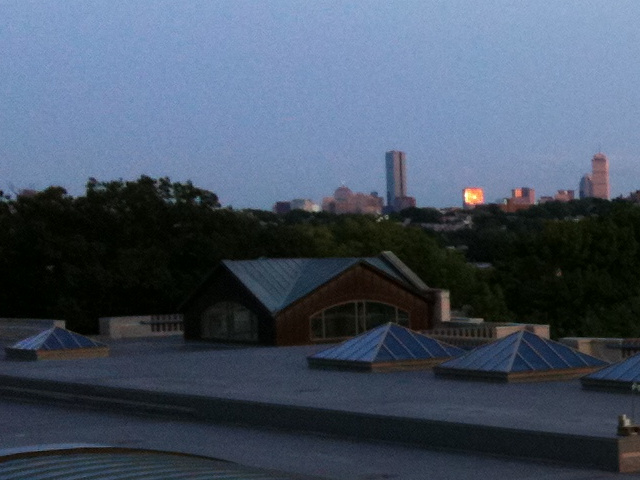
\includegraphics[width=.45\textwidth]{RooftopL001} \label{RooftopL}}
\subfigure{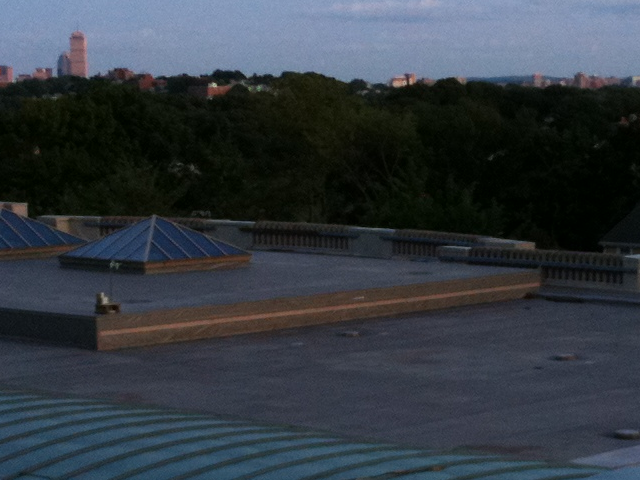
\includegraphics[width=.45\textwidth]{RooftopR001} \label{RooftopR}}
\caption{Rooftop Views (a) Left View, (b) Right View}
\end{figure}

\begin{figure}
\centering
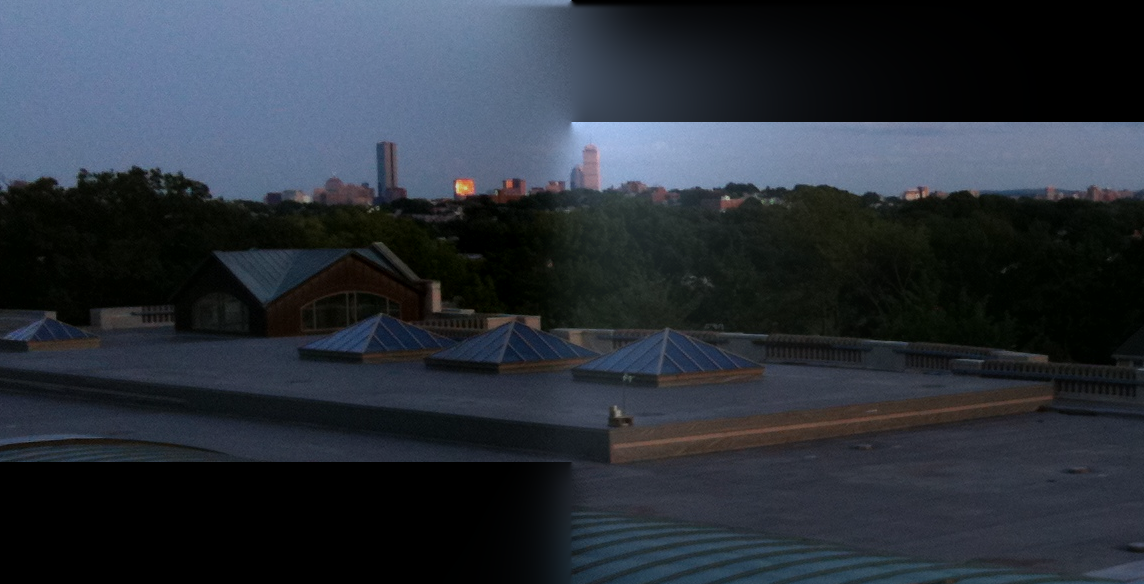
\includegraphics[width=1\textwidth]{RooftopSP001001}
\caption{Rooftop Views Blended}
\label{RooftopStitched}
\end{figure}

\begin{figure}
\centering
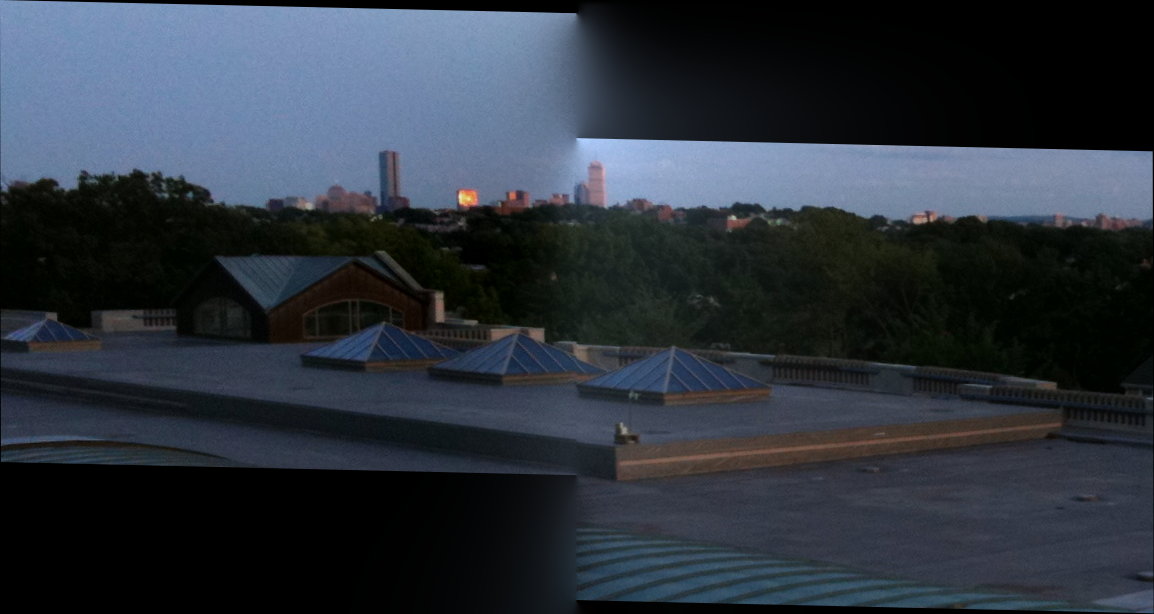
\includegraphics[width=1\textwidth]{RooftopSP001ManAff}
\caption{Rooftop Views Blended Manually (Affine)}
\label{RooftopStitchedManual}
\end{figure}

% ROOFTOP NOISE
\begin{figure}
\centering
\subfigure{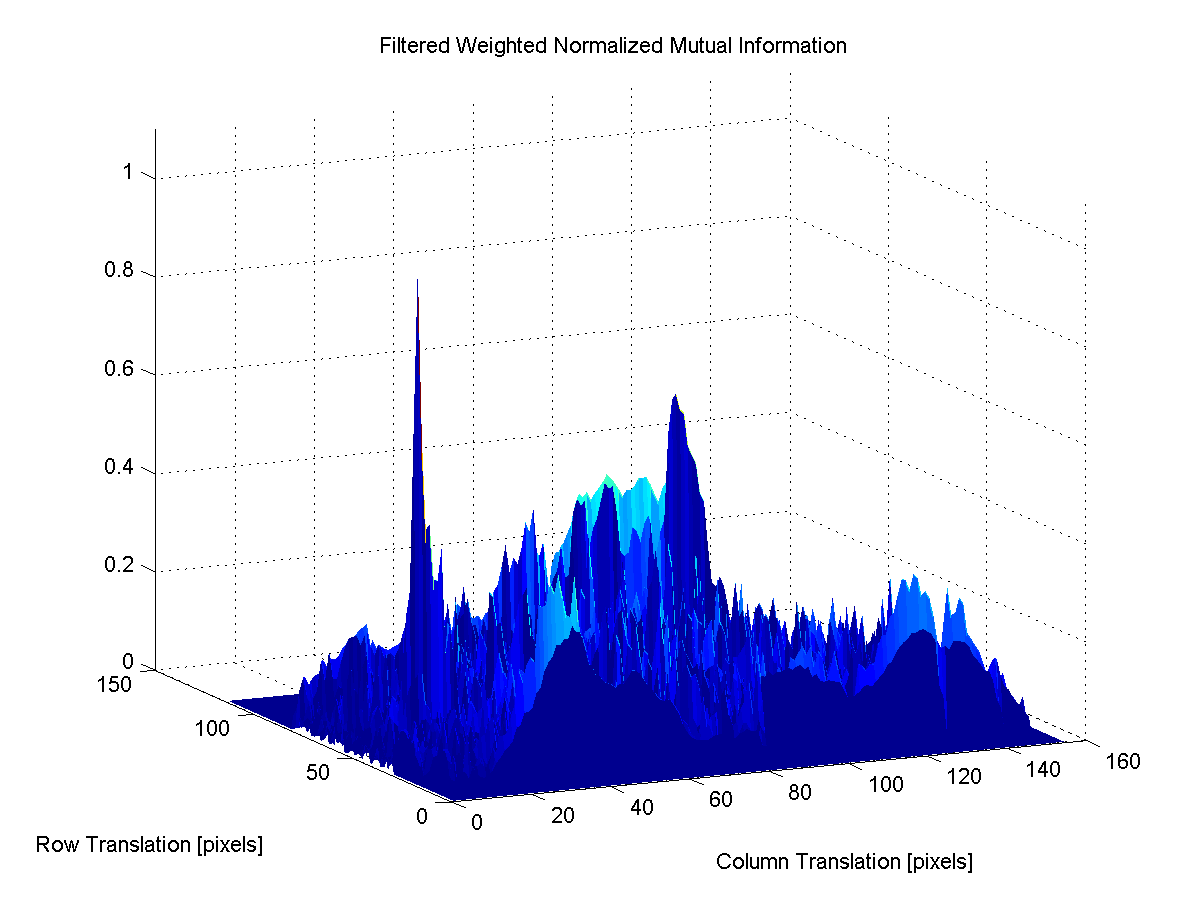
\includegraphics[width=.49\textwidth]{RooftopNoisy24122001FWNMI} \label{RooftopNoisy24122001FWNMI}}
\subfigure{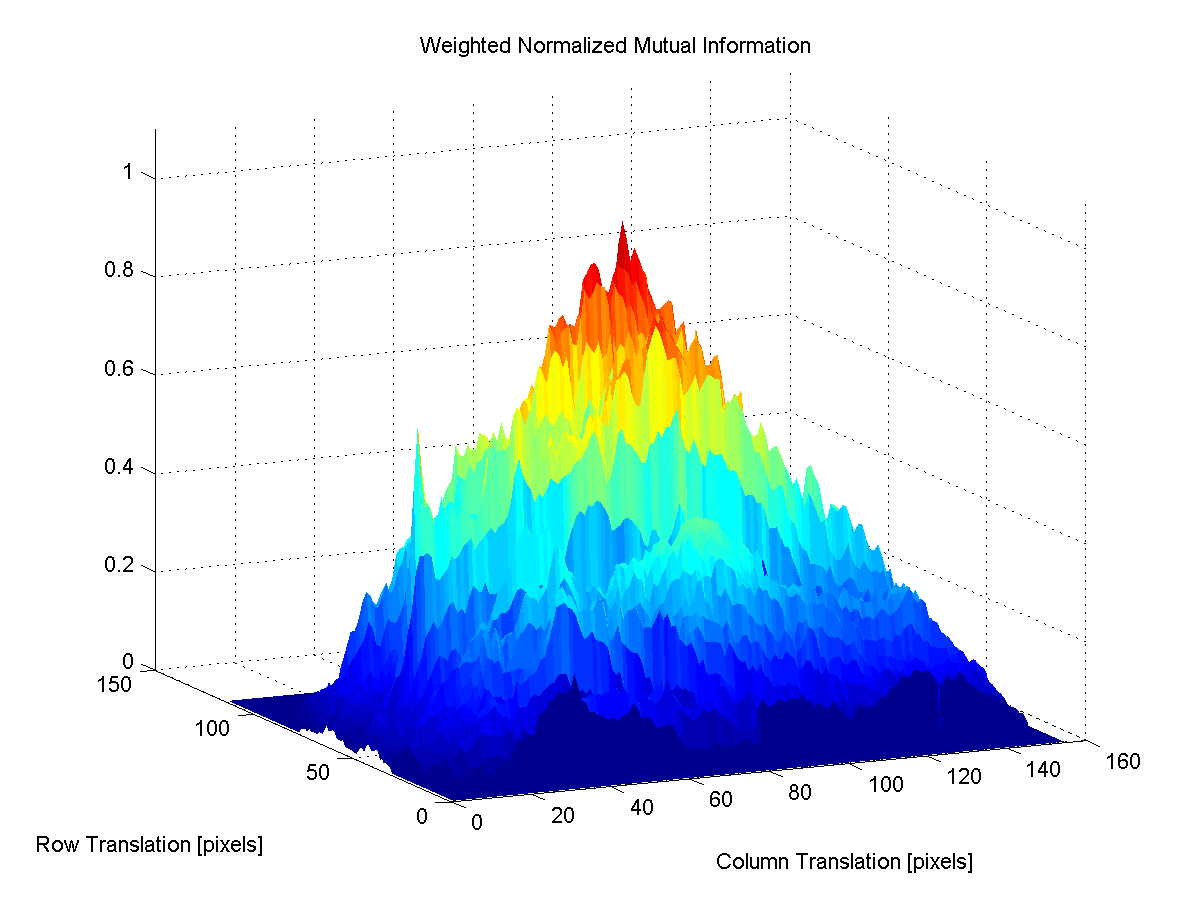
\includegraphics[width=.49\textwidth]{RooftopNoisy24122001WNMI} \label{RooftopNoisy24122001WNMI}}
\caption{Mutual Information Maps from Translation Search (a) Filtered and Weighted, (b) Weighted}
\label{RooftopNoisyImagesMI}
\end{figure}

\begin{figure}
\centering
\subfigure{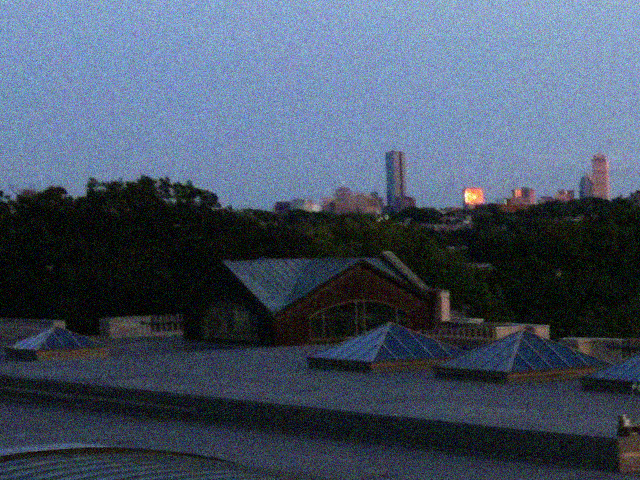
\includegraphics[width=.45\textwidth]{RooftopNoisy24122L001} \label{RooftopNoisy24122L001}}
\subfigure{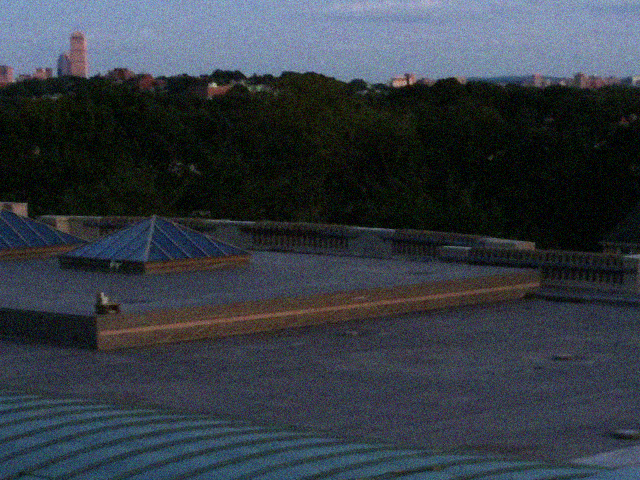
\includegraphics[width=.45\textwidth]{RooftopNoisy24122R001} \label{RooftopNoisy24122R001}}
\caption{Rooftop Views with Average SNR of 24.122 dB (a) Left View, (b) Right View}
\label{RooftopNoisyImages}
\end{figure}

\begin{figure}
\centering
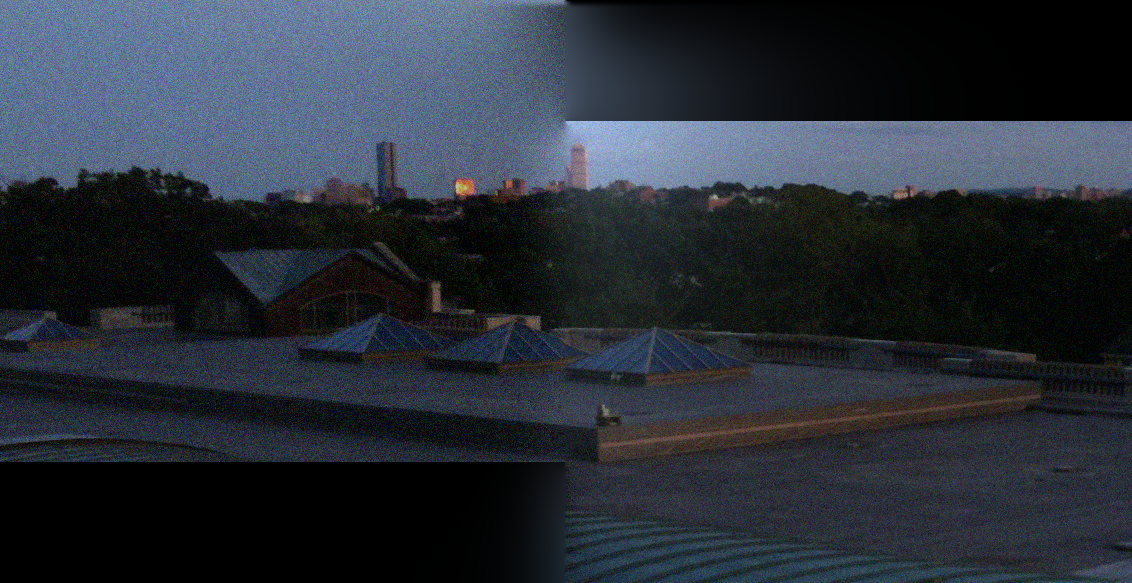
\includegraphics[width=1\textwidth]{RooftopNoisy24122SP001001}
\caption{Rooftop Noisy Views Blended (Average SNR: 24.122 dB)}
\label{RooftopNoisyStitched}
\end{figure}

% STONE WALL
\begin{figure}
\label{StoneWallImages}
\centering
\subfigure{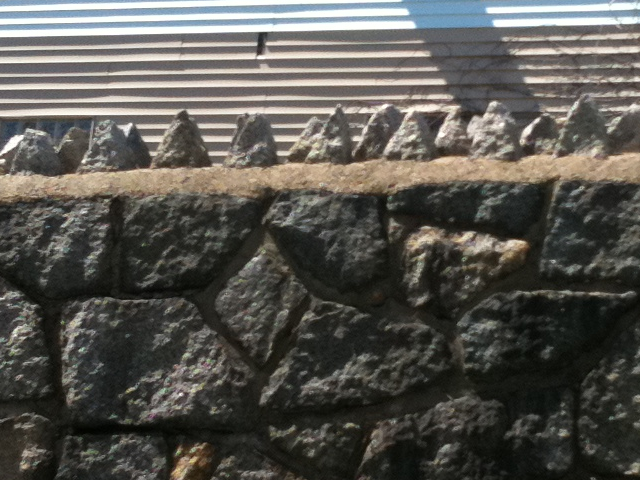
\includegraphics[width=.45\textwidth]{StoneWallL001} \label{StoneWallL}}
\subfigure{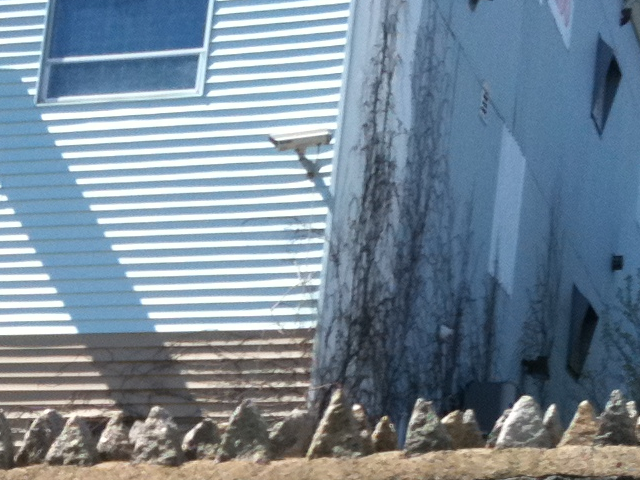
\includegraphics[width=.45\textwidth]{StoneWallR001} \label{StoneWallR}}
\caption{Stone Wall Scene (a) Left View, (b) Right View}
\end{figure}

\begin{figure}
\label{StoneWallStitched}
\centering
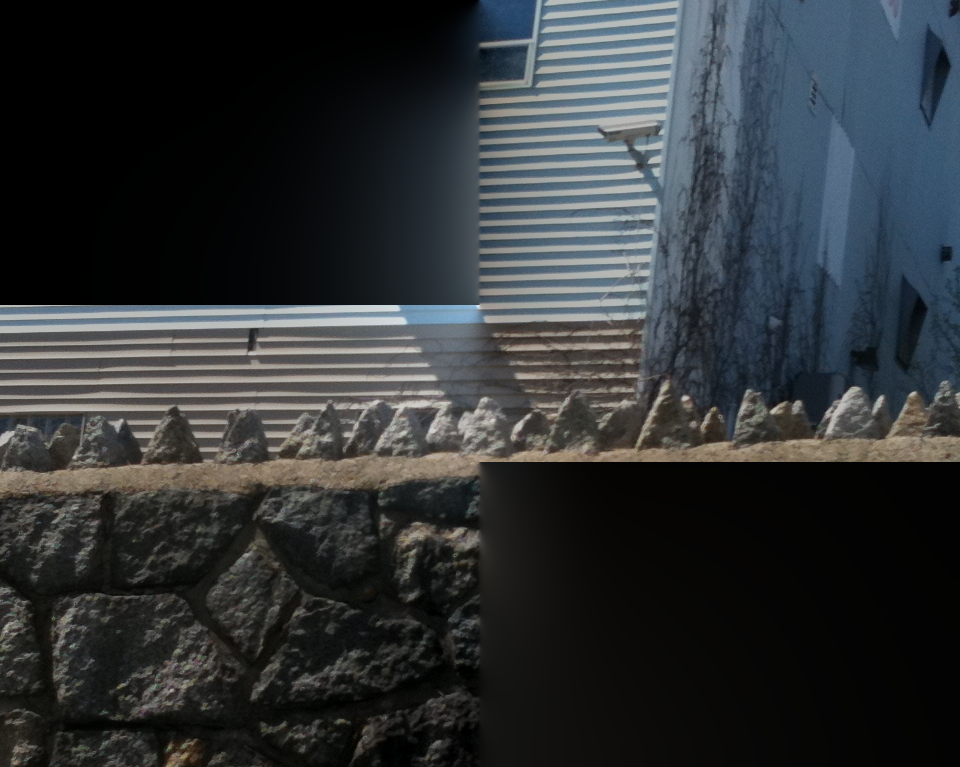
\includegraphics[width=1\textwidth]{StoneWallSP001001}
\caption{Stone Wall Views Blended}
\end{figure}

% STONEWALL NOISE
\begin{figure}
\centering
\subfigure{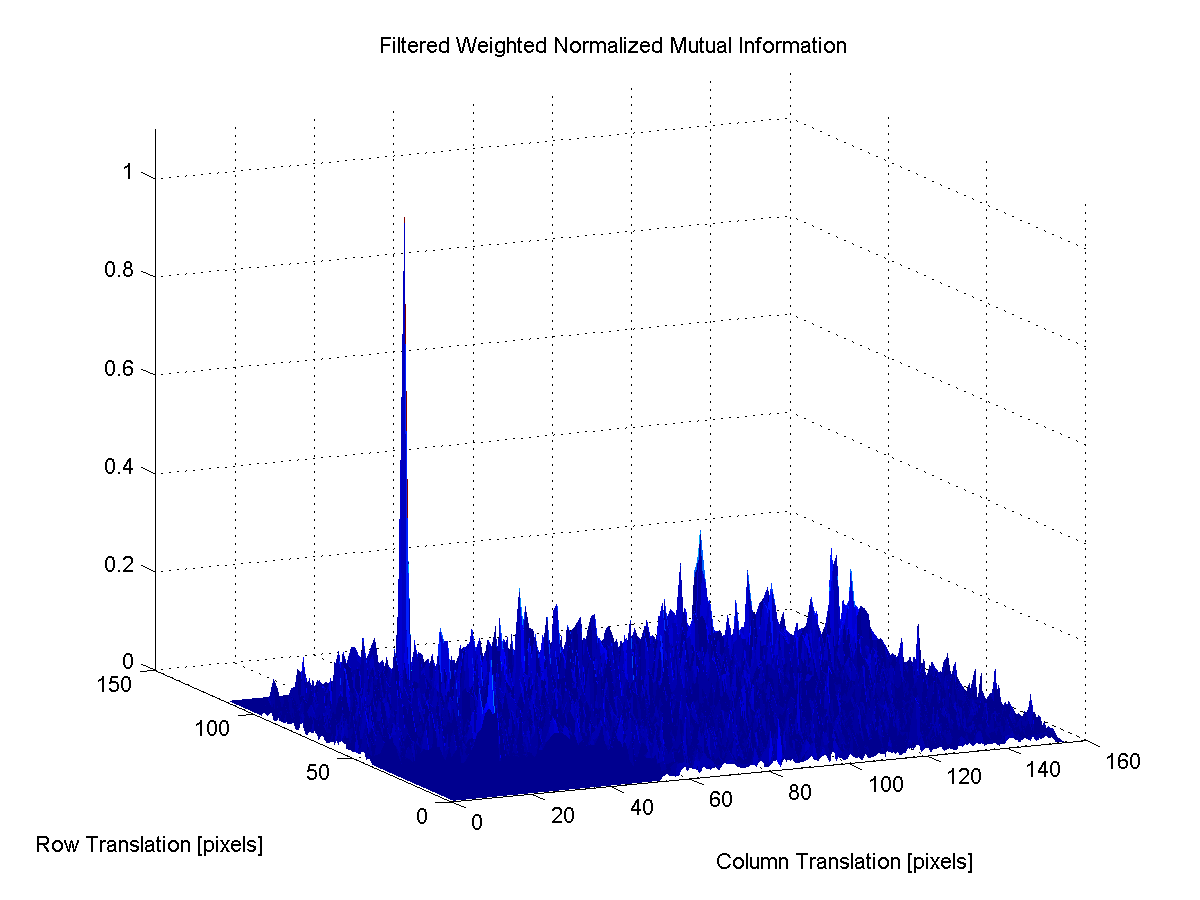
\includegraphics[width=.49\textwidth]{StoneWallNoisy164725001FWNMI} \label{StoneWallNoisy164725001FWNMI}}
\subfigure{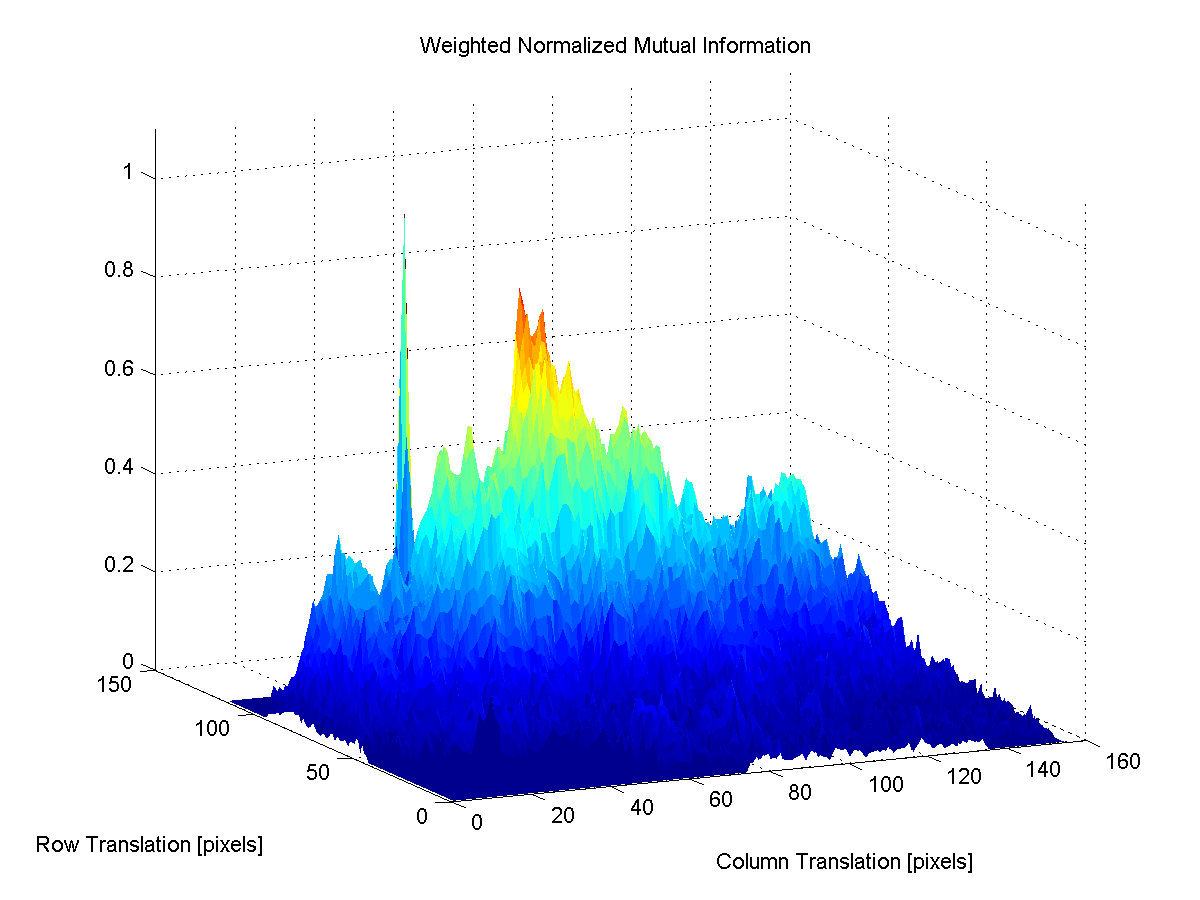
\includegraphics[width=.49\textwidth]{StoneWallNoisy164725001WNMI} \label{StoneWallNoisy164725001WNMI}}
\caption{Mutual Information Maps from Translation Search (a) Filtered and Weighted, (b) Weighted}
\label{StoneWallNoisyImagesMI}
\end{figure}

\begin{figure}
\centering
\subfigure{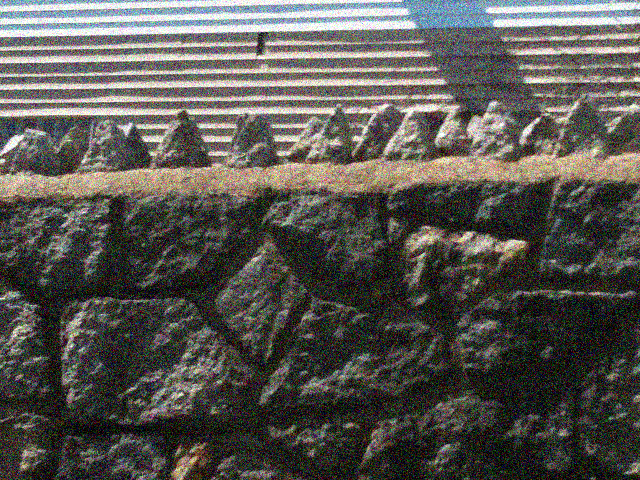
\includegraphics[width=.45\textwidth]{StoneWallNoisy164725L001} \label{StoneWallNoisy164725L001}}
\subfigure{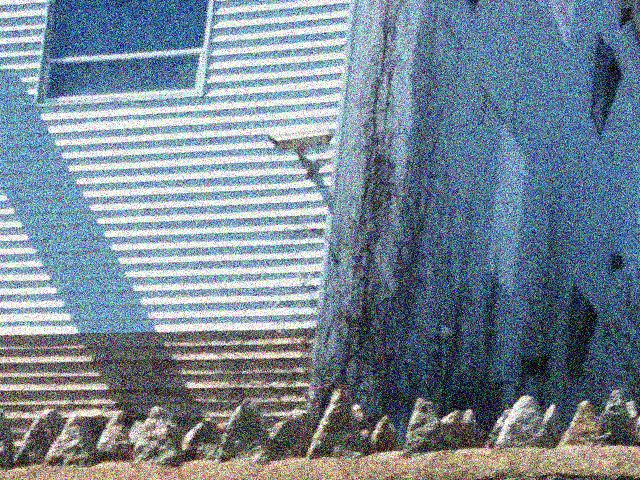
\includegraphics[width=.45\textwidth]{StoneWallNoisy164725R001} \label{StoneWallNoisy164725R001}}
\caption{Stone Wall Views with Average SNR of 16.473 dB (a) Left View, (b) Right View}
\label{StoneWallNoisyImages}
\end{figure}

\begin{figure}
\centering
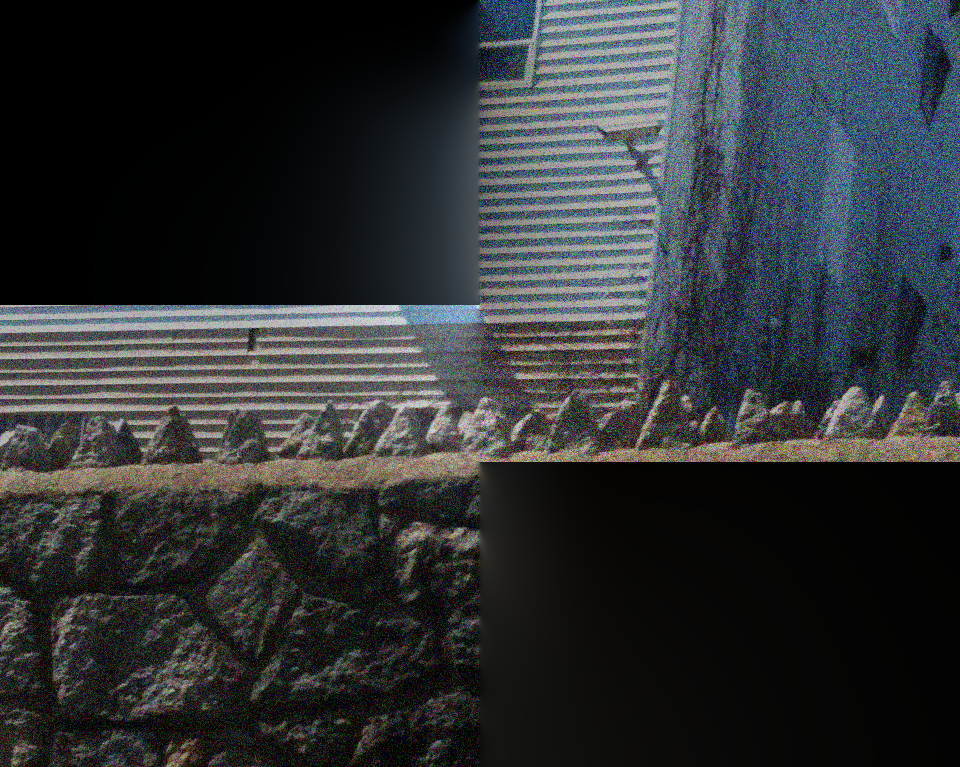
\includegraphics[width=1\textwidth]{StoneWallNoisy164725SP001001}
\caption{Stone Wall Noisy Views Blended (Average SNR: 16.473 dB)}
\label{StoneWallNoisyStitched}
\end{figure}

% STONEWALL SMALL OVERLAP
\begin{figure}
\centering
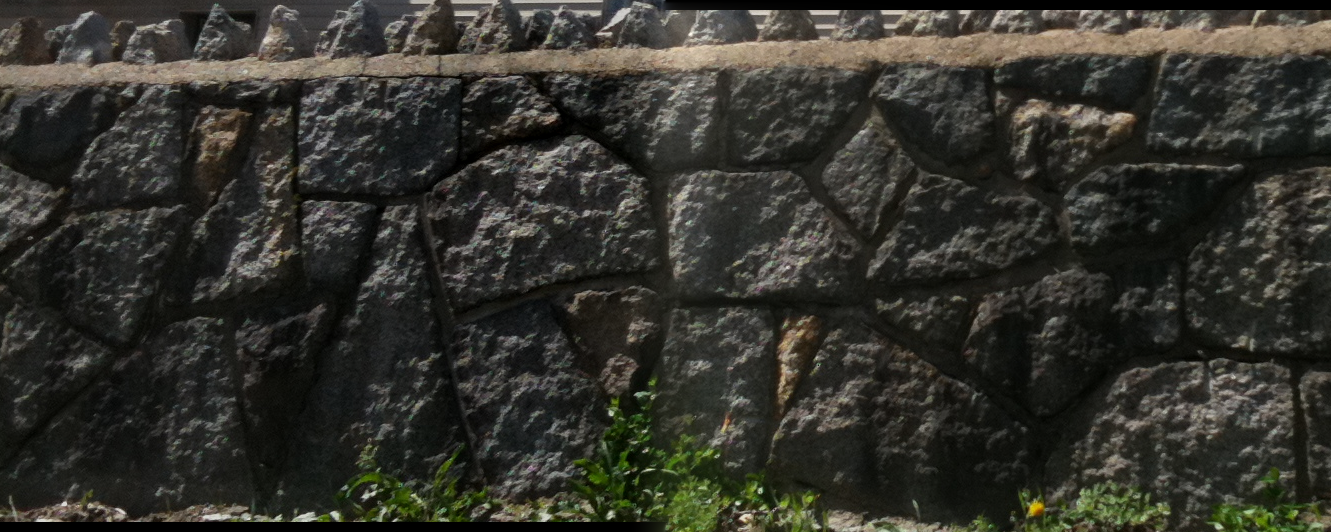
\includegraphics[width=.8\textwidth]{StoneWallSP002002}
\caption{Stone Wall Views Blended with 1\% Overlap}
\label{StoneWallSmall}
\end{figure}

%%%%%%%%%%%%%%%%%%%%%%%%%%%%%%%%%%%%%%%%%%%%%%%%%%%%%%%%%%%%%%%%%%%%%%%%%%%%%%%
% END OF DOCUMENT



%************************************
% SECTION 4.2
\section{Near-Affine Scenarios}

\indent
%%%%%%%%%%%%%%%%%%%%%%%%%%%%%%%%%%%%%%%%%%%%%%%%%%%%%%%%%%%%%%%%%%%%%%%%%%%%%%%
%
% Tommy P. Keane
% Master of Science Thesis
% Department of Electrical and Microelectronic Engineering
%
% March 2011
%
%
%
% .tex and .sty modified from:
% http://www.ce.rit.edu/studentresources/gradresource/LaTexThesis.zip
%
%%%%%%%%%%%%%%%%%%%%%%%%%%%%%%%%%%%%%%%%%%%%%%%%%%%%%%%%%%%%%%%%%%%%%%%%%%%%%%%

%%%%%%%%%%%%%%%%%%%%%%%%%%%%%%%%%%%%%%%%%%%%%%%%%%%%%%%%%%%%%%%%%%%%%%%%%%%%%%%
%
% CHAPTER 2
%
% SECTION 2
%
%%%%%%%%%%%%%%%%%%%%%%%%%%%%%%%%%%%%%%%%%%%%%%%%%%%%%%%%%%%%%%%%%%%%%%%%%%%%%%%


%%%%%%%%%%%%%%%%%%%%%%%%%%%%%%%%%%%%%%%%%%%%%%%%%%%%%%%%%%%%%%%%%%%%%%%%%%%%%%%
% BEGIN DOCUMENT




%%%%%%%%%%%%%%%%%%%%%%%%%%%%%%%%%%%%%%%%%%%%%%%%%%%%%%%%%%%%%%%%%%%%%%%%%%%%%%%
% END OF DOCUMENT




%************************************
% SECTION 4.3
\section{Projective Scenarios}

\indent
%%%%%%%%%%%%%%%%%%%%%%%%%%%%%%%%%%%%%%%%%%%%%%%%%%%%%%%%%%%%%%%%%%%%%%%%%%%%%%%
%
% Tommy P. Keane
% Master of Science Thesis
% Department of Electrical and Microelectronic Engineering
%
% March 2011
%
%
%
% .tex and .sty modified from:
% http://www.ce.rit.edu/studentresources/gradresource/LaTexThesis.zip
%
%%%%%%%%%%%%%%%%%%%%%%%%%%%%%%%%%%%%%%%%%%%%%%%%%%%%%%%%%%%%%%%%%%%%%%%%%%%%%%%

%%%%%%%%%%%%%%%%%%%%%%%%%%%%%%%%%%%%%%%%%%%%%%%%%%%%%%%%%%%%%%%%%%%%%%%%%%%%%%%
%
% CHAPTER 4
%
% SECTION 3: Complex Views
%
%%%%%%%%%%%%%%%%%%%%%%%%%%%%%%%%%%%%%%%%%%%%%%%%%%%%%%%%%%%%%%%%%%%%%%%%%%%%%%%


%%%%%%%%%%%%%%%%%%%%%%%%%%%%%%%%%%%%%%%%%%%%%%%%%%%%%%%%%%%%%%%%%%%%%%%%%%%%%%%
% BEGIN DOCUMENT

TO BE WRITTEN

% ART GALLERY 001
\begin{figure}[h]
\centering
\subfigure{ 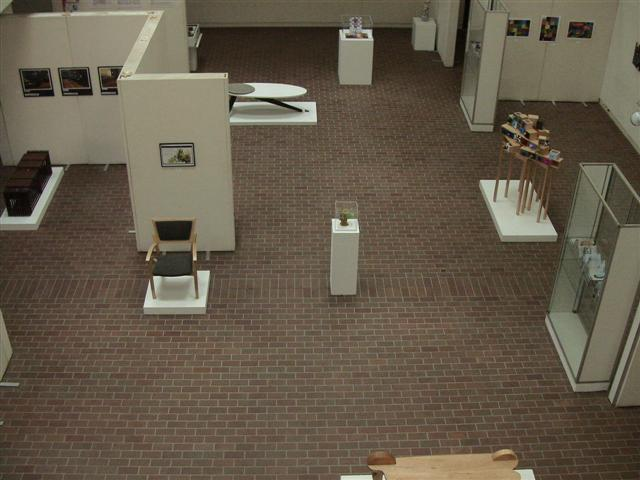
\includegraphics[width=.45\textwidth]{AGS1L001} \label{ArtGallery1L} }
\subfigure{ 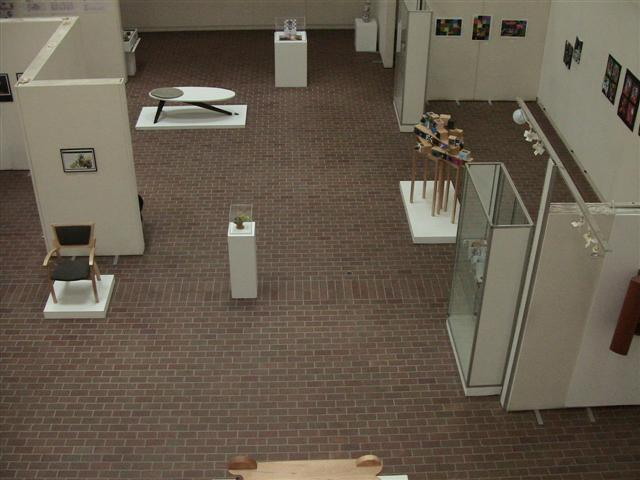
\includegraphics[width=.45\textwidth]{AGS1R001} \label{ArtGallery1R} }
\caption{Art Gallery Scene 01 (a) Left View, (b) Right View}
\label{ArtGallery1Images}
\end{figure}

\begin{figure}[h]
\centering
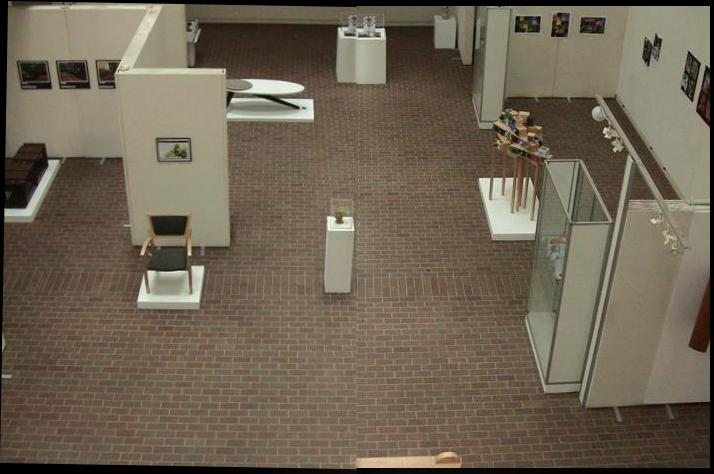
\includegraphics[width=1\textwidth]{AGS1SP001001}
\caption{Art Gallery 01 Views Blended}
\label{ArtGallery1Stitched}
\end{figure}




% ART GALLERY 002
\begin{figure}[h]
\centering
\subfigure{ 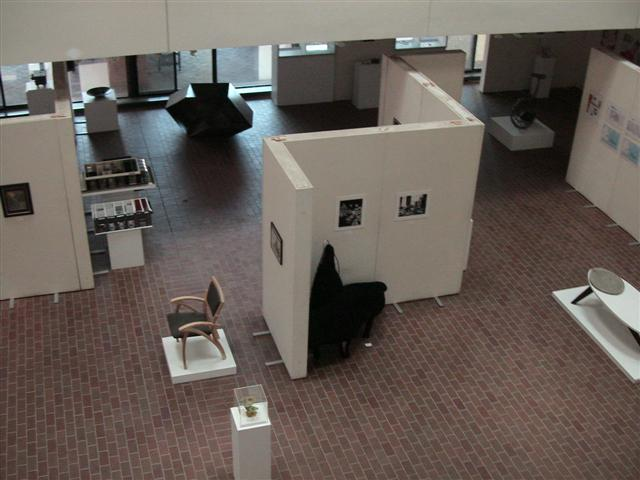
\includegraphics[width=.45\textwidth]{AGS2L001} \label{ArtGallery2L} }
\subfigure{ 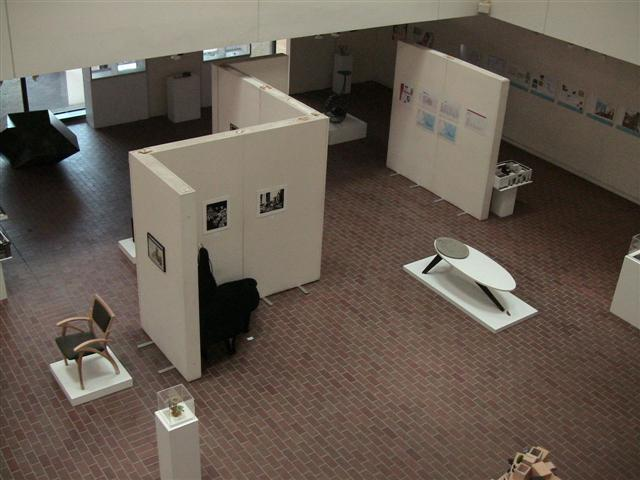
\includegraphics[width=.45\textwidth]{AGS2R001} \label{ArtGallery2R} }
\caption{Art Gallery Scene 02 (a) Left View, (b) Right View}
\label{ArtGallery2Images}
\end{figure}

\begin{figure}[h]
\label{ArtGallery2Stitched}
\centering
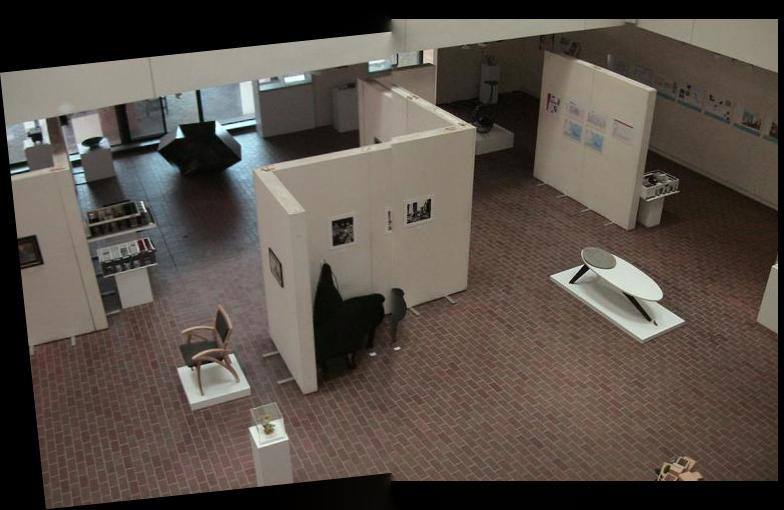
\includegraphics[width=1\textwidth]{AGS2SP001001}
\caption{Art Gallery 02 Views Blended}
\end{figure}



% LENEL 005
\begin{figure}[h]
\centering
\subfigure{ 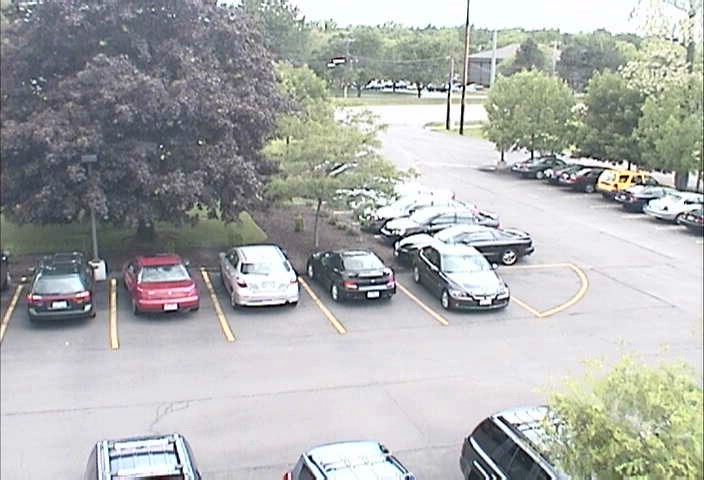
\includegraphics[width=.45\textwidth]{Lenel005L001} \label{Lenel5L} }
\subfigure{ 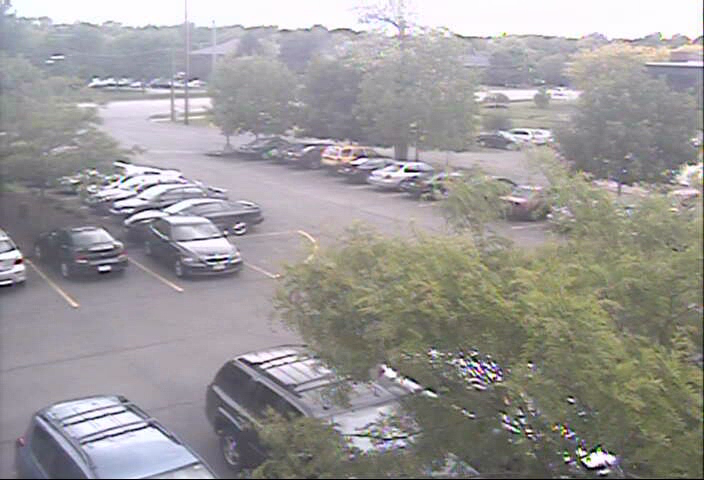
\includegraphics[width=.45\textwidth]{Lenel005R001} \label{Lenel5R} }
\caption{Lenel Front Lot Scene (a) Left View, (b) Right View}
\label{Lenel5Images}
\end{figure}

\begin{figure}[h]
\centering
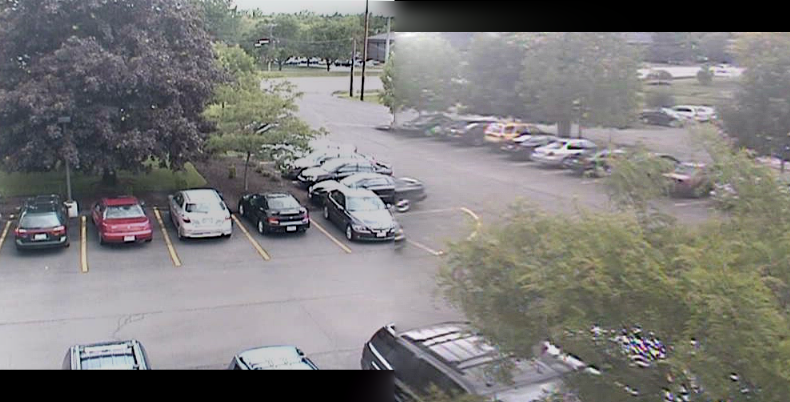
\includegraphics[width=1\textwidth]{Lenel005SP001001}
\caption{Lenel Front Lot Views Blended}
\label{Lenel5Stitched}
\end{figure}



% LENEL 010
\begin{figure}[h]
\centering
\subfigure{ 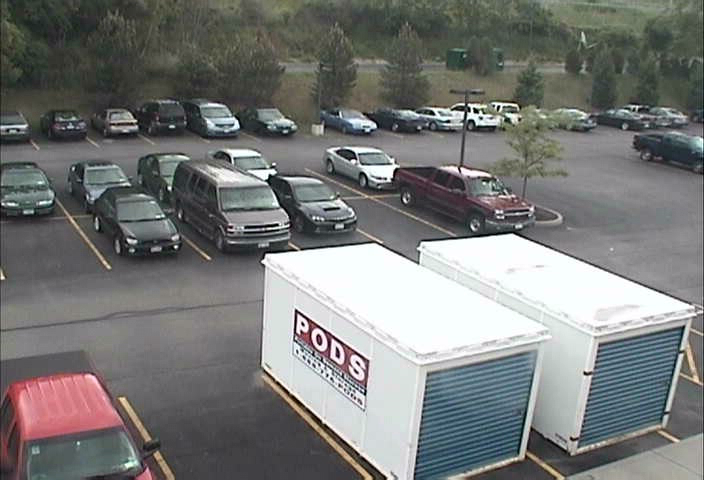
\includegraphics[width=.45\textwidth]{Lenel010L004} \label{Lenel10L} }
\subfigure{ 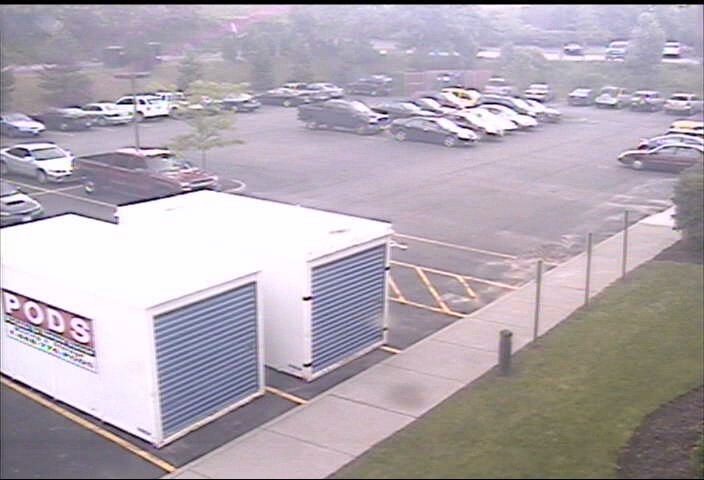
\includegraphics[width=.45\textwidth]{Lenel010R004} \label{Lenel10R} }
\caption{Lenel Back Lot Scene (a) Left View, (b) Right View}
\label{Lenel10Images}
\end{figure}

\begin{figure}[h]
\centering
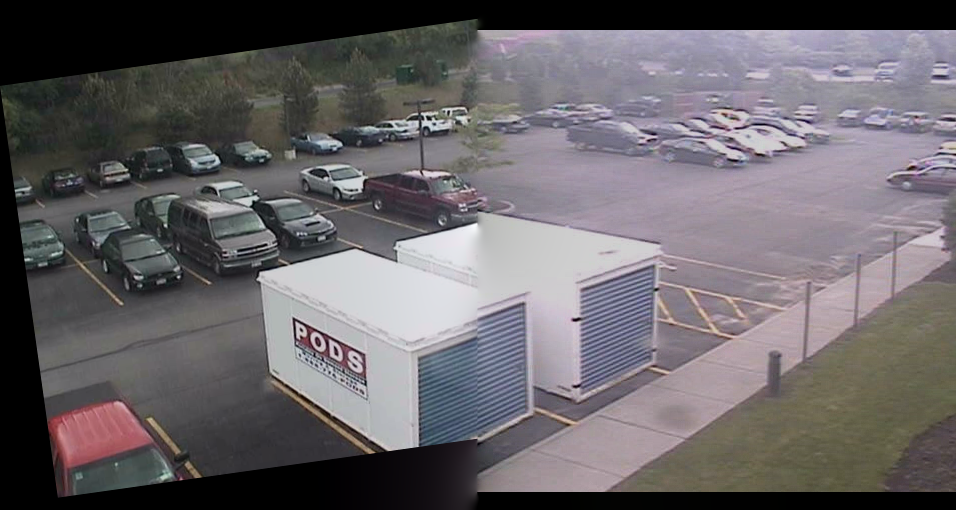
\includegraphics[width=1\textwidth]{Lenel010SP001}
\caption{Lenel Back Lot Views Blended}
\label{Lenel10Stitched}
\end{figure}


%%%%%%%%%%%%%%%%%%%%%%%%%%%%%%%%%%%%%%%%%%%%%%%%%%%%%%%%%%%%%%%%%%%%%%%%%%%%%%%
% END OF DOCUMENT






%%%%%%%%%%%%%%%%%%%%%%%%%%%%%%%%%%%%%%%%%%%%%%%%%%%%%%%%%%%%%%%%%%%%%%%%%%%%%%%
% CHAPTER 5
\chapter{Conclusions and Future Work}

\indent
%%%%%%%%%%%%%%%%%%%%%%%%%%%%%%%%%%%%%%%%%%%%%%%%%%%%%%%%%%%%%%%%%%%%%%%%%%%%%%%
%
% Tommy P. Keane
% Master of Science Thesis
% Department of Electrical and Microelectronic Engineering
%
% March 2011
%
%
%
% .tex and .sty modified from:
% http://www.ce.rit.edu/studentresources/gradresource/LaTexThesis.zip
%
%%%%%%%%%%%%%%%%%%%%%%%%%%%%%%%%%%%%%%%%%%%%%%%%%%%%%%%%%%%%%%%%%%%%%%%%%%%%%%%

%%%%%%%%%%%%%%%%%%%%%%%%%%%%%%%%%%%%%%%%%%%%%%%%%%%%%%%%%%%%%%%%%%%%%%%%%%%%%%%
%
% CHAPTER 6
%
% PREAMBLE
%
%%%%%%%%%%%%%%%%%%%%%%%%%%%%%%%%%%%%%%%%%%%%%%%%%%%%%%%%%%%%%%%%%%%%%%%%%%%%%%%


%%%%%%%%%%%%%%%%%%%%%%%%%%%%%%%%%%%%%%%%%%%%%%%%%%%%%%%%%%%%%%%%%%%%%%%%%%%%%%%
% BEGIN DOCUMENT

The presented algorithm generates convincing panoramic views automatically for complex scenes. The research here has investigated the robustness of mutual information as a metric for complex, realistic scenes. There is still a large amount of room for improvement, but this work has shown the strength and versatility of mutual information, especially for overcoming difficult problems such as parallax differences and object occlusions between multiple views. In the case of occlusion it is important to keep in mind that there is no perfect registration as portions of the scene are available in one view but not in the other(s). In these cases, the best registration would be the one that can correspond the pixels of objects that exist in both views. This scenario is the prime case for the strength of the WFMI algorithm, since there is not a reliance on sparse pixel-to-pixel correspondences, but rather segment-to-segment correspondence. Therefore, occlusion is not a crippling problem for the WFMI registration algorithm. In the case of parallax differences between views and the complexities arising from the projective geometry of multi-view imaging, the appropriate homography may not exist and a Fundamental matrix or a non-linear polynomial mapping may be more appropriate. Categorizing these scenarios as Projective in nature (as in: related by a projective homography) was shown as an appropriate simplification in the manual registration examples, but the WFMI algorithm has shown that the even further simplification to the affine search-space can still produce accurate registration, or an appropriate estimate in the more complex scenarios.

%%%%%%%%%%%%%%%%%%%%%%%%%%%%%%%%%%%%%%%%%%%%%%%%%%%%%%%%%%%%%%%%%%%%%%%%%%%%%%%
% END OF DOCUMENT


%************************************
% SECTION 5.1
\section{Future Work}

\indent
%%%%%%%%%%%%%%%%%%%%%%%%%%%%%%%%%%%%%%%%%%%%%%%%%%%%%%%%%%%%%%%%%%%%%%%%%%%%%%%
%
% Tommy P. Keane
% Master of Science Thesis
% Department of Electrical and Microelectronic Engineering
% Rochester Institute of Technology
%
% April 2011
%
%
%
% Funded By: Lenel Systems Inc., A UTC Fire & Security Corporation
%
% Algorithm Intellectual Property Owned By: Lenel Systems Inc.
%
%
% http://www.tommypkeane.com
%
%%%%%%%%%%%%%%%%%%%%%%%%%%%%%%%%%%%%%%%%%%%%%%%%%%%%%%%%%%%%%%%%%%%%%%%%%%%%%%%

%%%%%%%%%%%%%%%%%%%%%%%%%%%%%%%%%%%%%%%%%%%%%%%%%%%%%%%%%%%%%%%%%%%%%%%%%%%%%%%
%
% CHAPTER 6
%
% SECTION 1
%
%%%%%%%%%%%%%%%%%%%%%%%%%%%%%%%%%%%%%%%%%%%%%%%%%%%%%%%%%%%%%%%%%%%%%%%%%%%%%%%


%%%%%%%%%%%%%%%%%%%%%%%%%%%%%%%%%%%%%%%%%%%%%%%%%%%%%%%%%%%%%%%%%%%%%%%%%%%%%%%
% BEGIN DOCUMENT

Originally this work was set out as a project to replace a system of manual image registration for surveillance videos by means of a fully automatic software implementation utilizing stationary cameras with unknown locations and no \textit{a priori} information, besides allowing for the assumption of some amount of overlap between views that can be registered. The complexity of the scenario and project guidelines went beyond the initial scope of the project, but the novel application of mutual information was introduced and tested. An initial expansion of the algorithm would be to finalize the registration for non-affine views by enhancing the algorithm with a pixel-to-pixel correspondence algorithm applied to the determined overlap region. Given that the WFMI algorithm provides intelligent estimates for the registration of views of complex scenes, relatively simple registration algorithms could be successful when applied to the estimated overlap region. In this respect the WFMI algorithm would be setting initial conditions to limit the search space for pixel-based registration, allowing for faster and more efficient computations in robust registration algorithms. In a practical implementation, the WFMI algorithm could provide an initial estimate on video feed frames and as more frames are calculated, refinements could be made to the initial estimate, especially as objects pass through the overlap regions of the views being registered.

There was also some initial research done in investigating the application of unsupervised image segmentation, such as the robust and accurate algorithm in \cite{Ugarriza2009}, to generate better features for object correspondence. Again, since the WFMI algorithm is a region-based registration, the more intelligently that features are generated to define object boundaries rather than intensity data, the more accurate the mutual information metric will be, as overlapping segments containing the same object will be a relatively unique statistical event sharing the same feature histograms. However, this could greatly increase computational complexity as the segmentation would need to be robust considering the practical scenarios: uncontrolled weather, illumination, and camera artifacts.

In terms of advancing the application of the weighted and filtered mutual information metric itself, there is a lot of contemporary research moving towards scene understanding and 3-dimensional (spatial) image and video data. Multiple views of a scene directly allow for the extension of the projective geometry to develop 3-D information about the structure of the scene, and the objects within it. If a scene's structure is unknown from its views and an accurate registration is not available, the WFMI metric could be applied to identify objects, regions, or even elements of the scene in motion that are correlated between the views. Object tracking, depth reconstruction, and motion estimation could all be rich areas of research for this novel application of information theory.

%%%%%%%%%%%%%%%%%%%%%%%%%%%%%%%%%%%%%%%%%%%%%%%%%%%%%%%%%%%%%%%%%%%%%%%%%%%%%%%
% END OF DOCUMENT


%************************************
% SECTION 5.2
\section{Final Remarks}

\indent
%%%%%%%%%%%%%%%%%%%%%%%%%%%%%%%%%%%%%%%%%%%%%%%%%%%%%%%%%%%%%%%%%%%%%%%%%%%%%%%
%
% Tommy P. Keane
% Master of Science Thesis
% Department of Electrical and Microelectronic Engineering
%
% March 2011
%
%
%
% .tex and .sty modified from:
% http://www.ce.rit.edu/studentresources/gradresource/LaTexThesis.zip
%
%%%%%%%%%%%%%%%%%%%%%%%%%%%%%%%%%%%%%%%%%%%%%%%%%%%%%%%%%%%%%%%%%%%%%%%%%%%%%%%

%%%%%%%%%%%%%%%%%%%%%%%%%%%%%%%%%%%%%%%%%%%%%%%%%%%%%%%%%%%%%%%%%%%%%%%%%%%%%%%
%
% CHAPTER 5
%
% SECTION 2
%
%%%%%%%%%%%%%%%%%%%%%%%%%%%%%%%%%%%%%%%%%%%%%%%%%%%%%%%%%%%%%%%%%%%%%%%%%%%%%%%


%%%%%%%%%%%%%%%%%%%%%%%%%%%%%%%%%%%%%%%%%%%%%%%%%%%%%%%%%%%%%%%%%%%%%%%%%%%%%%%
% BEGIN DOCUMENT

TO BE WRITTEN

% ART GALLERY 4
\begin{figure}[!h]
\label{ArtGallery4Images}
\centering
\subfigure{ 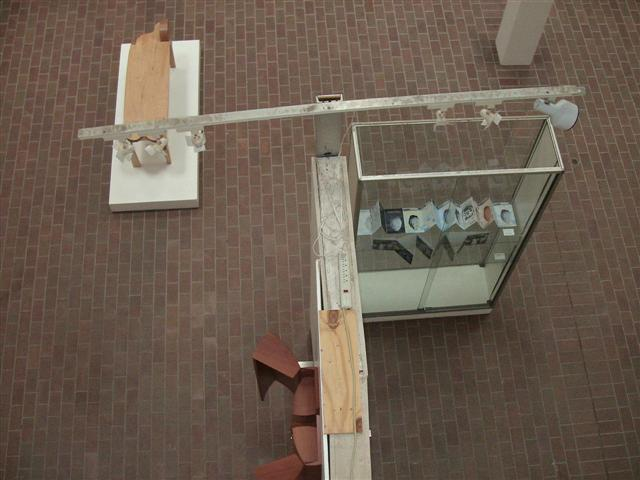
\includegraphics[width=.4\textwidth]{AGS4L005} \label{ArtGallery4L} }
\subfigure{ 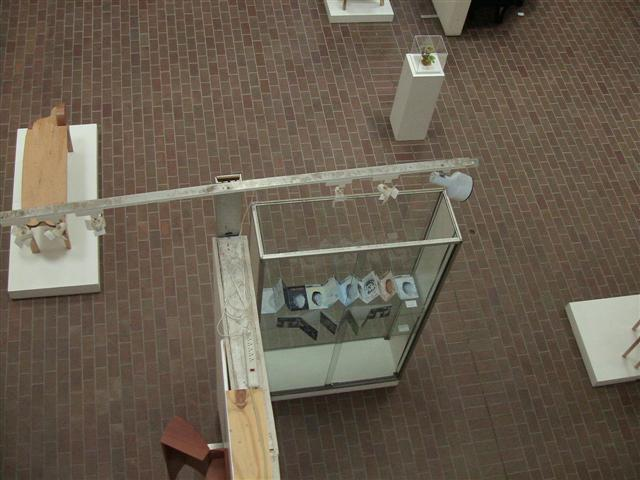
\includegraphics[width=.4\textwidth]{AGS4R005} \label{ArtGallery4R} }
\caption{Art Gallery 04 Scene (a) Left View, (b) Right View}
\end{figure}

\begin{figure}[!h]
\label{ArtGallery4Stitched}
\centering
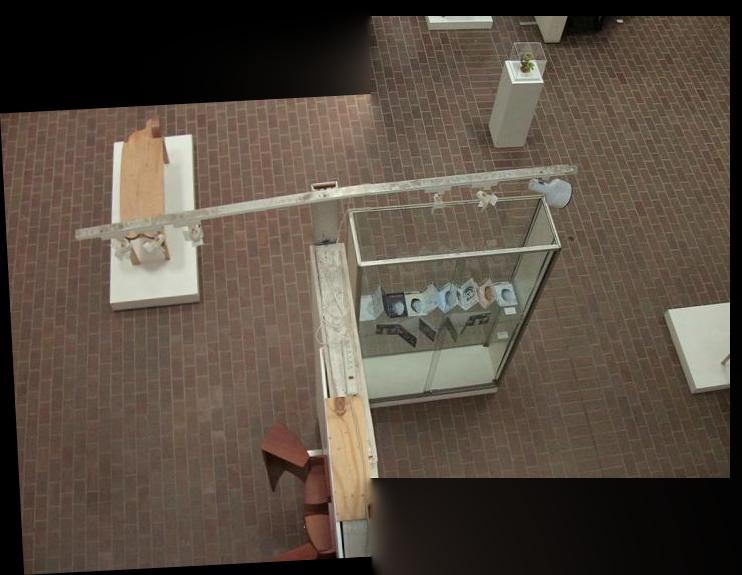
\includegraphics[width=1\textwidth]{AGS4SP005005}
\caption{Art Gallery 04 Views Blended}
\end{figure}

\begin{figure}[!h]
\label{ArtGallery4StitchedManual}
\centering
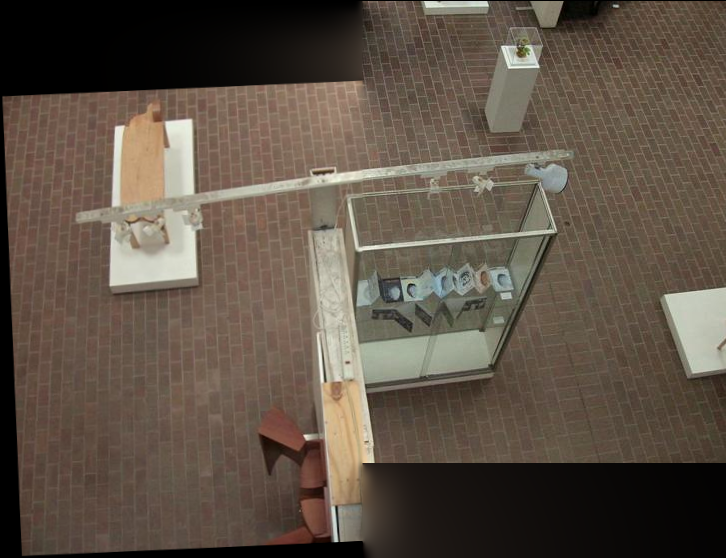
\includegraphics[width=1\textwidth]{AGS4SP005ManAff}
\caption{Art Gallery 04 Views Blended Manually (Affine)}
\end{figure}



%%%%%%%%%%%%%%%%%%%%%%%%%%%%%%%%%%%%%%%%%%%%%%%%%%%%%%%%%%%%%%%%%%%%%%%%%%%%%%%
% END OF DOCUMENT




\end{doublespace}

%%%%%%%%%%%%%%%%%%%%%%%%%%%%%%%%%%%%%%%%%%%%%%%%%%%%%%%%%%%%%%%%%%%%%%%%%%%%%%%
% REFERENCES
\begin{singlespace}
	\bibliography{TommyKeane_MS_Thesis_Bibliography.bib}
	\nocite{*}
\end{singlespace}


%%%%%%%%%%%%%%%%%%%%%%%%%%%%%%%%%%%%%%%%%%%%%%%%%%%%%%%%%%%%%%%%%%%%%%%%%%%%%%%
% END OF DOCUMENT
\end{document}
